\documentclass[a4paper,12]{article}
\usepackage{amsmath, amsfonts, amssymb, amsthm, bm, graphics, bbm, color}
\usepackage{graphicx}
\usepackage{subfigure}
\usepackage{mathtools}
\usepackage[table]{xcolor}
\usepackage{url}
\usepackage{mathabx}
\usepackage{cancel}
\usepackage{multicol}
\usepackage{float}
\usepackage{caption}
\usepackage{mathalfa}
\usepackage{hyperref}
\usepackage{fancyvrb}
\usepackage{listings}
%\usepackage{unicode-math}
\captionsetup{font=footnotesize}
\captionsetup{width=\textwidth}
\DeclareMathAlphabet\mathbfcal{OMS}{cmsy}{b}{n}
\newtheorem{theorem}{Theorem}[section]
\newtheorem{lemma}[theorem]{Lemma}
\newtheorem{Corollary}[theorem]{Corollary}
\newtheorem{proposition}[theorem]{Proposition}
\theoremstyle{definition}
\newtheorem{definition}[theorem]{Definition}
\newtheorem{example}[theorem]{Example}

\newcommand\y{\cellcolor{gray!50}}

\newcommand\p{\cellcolor{gray!25}}

\makeatletter
\newcommand\makebig[2]{%
  \@xp\newcommand\@xp*\csname#1\endcsname{\bBigg@{#2}}%
  \@xp\newcommand\@xp*\csname#1l\endcsname{\@xp\mathopen\csname#1\endcsname}%
  \@xp\newcommand\@xp*\csname#1r\endcsname{\@xp\mathclose\csname#1\endcsname}%
}
\makeatother

\makebig{biggg} {3.0}
\makebig{Biggg} {3.5}
\makebig{bigggg}{4.0}
\makebig{Bigggg}{4.5}
\makebig{biggggg}{5.0}
\makebig{Biggggg}{5.5}
\makebig{bigggggg}{6.0}
\makebig{Bigggggg}{6.5}

\newcommand\bovermat[2]{%
    \makebox[0pt][l]{$\smash{\overbrace{\phantom{%
                    \begin{matrix}#2\end{matrix}}}^{\text{#1}}}$}#2}

\newcommand\bundermat[2]{%
    \makebox[0pt][l]{$\smash{\underbrace{\phantom{%
                    \begin{matrix}#2\end{matrix}}}_{\text{#1}}}$}#2}

\newcommand\partialphantom{\vphantom{\frac{\partial e_{P,M}}{\partial w_{1,1}}}}


\newcommand{\raisesym}[2]{\raisebox{0.5\depth}{$#1\Biggggg \}$}}

\makeatletter
\newcommand*{\shifttext}[2]{%
  \settowidth{\@tempdima}{#2}%
  \makebox[\@tempdima]{\hspace*{#1}#2}%
}

% redefine paper size
\setlength{\oddsidemargin}{0in}
\setlength{\textwidth}{6.4in}
\setlength{\topmargin}{-0.5in}
\setlength{\textheight}{9.9in}
\setlength{\headheight}{0in}

\newcommand{\dif}{\mathrm{d}}
\newcommand{\im}{\mathrm{i}}


% Defining unicode characters for tree
\usepackage[utf8]{inputenc}
\usepackage{newunicodechar}
\makeatletter
\verbatim@font
\newsavebox\v@sp
\sbox{\v@sp}{\ }
\newlength{\v@spwd}
\setlength{\v@spwd}{\wd\v@sp}
\newunicodechar{└}{\mbox{\kern0.5\v@spwd\vrule height 2ex depth -1ex width 0.2ex\kern-0.2ex\rule[1ex]{0.5\v@spwd}{0.2ex}}}
\newunicodechar{─}{\rule[1ex]{1\v@spwd}{0.2ex}}
\newunicodechar{┬}{\rule[1ex]{0.5\v@spwd}{0.2ex}\vrule height 1ex
depth 0.5ex width0.2ex\kern-0.2ex\rule[1ex]{0.5\v@spwd}{0.2ex}}
\newunicodechar{├}{\mbox{\kern0.5\v@spwd\vrule height 2ex depth 0.5ex width 0.2ex\kern-0.2ex\rule[1ex]{0.5\v@spwd}{0.2ex}}}
\newunicodechar{│}{\mbox{\kern0.5\v@spwd\vrule height 2ex depth 0.5ex width
0.2ex\kern-0.2ex \kern0.5\v@spwd}}
\makeatother
\normalfont

% Defining code style:
\definecolor{codegreen}{rgb}{0,0.6,0}
\definecolor{codegray}{rgb}{0.5,0.5,0.5}
\definecolor{codepurple}{rgb}{0.58,0,0.82}
\definecolor{backcolour}{rgb}{0.95,0.92,0.92}

% 1. General Python Keywords List
\lstdefinelanguage{PythonPlus}[]{Python}{
  morekeywords=[1]{,as,assert,nonlocal,with,yield,self,True,False,None,} % Python builtin
  morekeywords=[2]{,__init__,__add__,__mul__,__div__,__sub__,__call__,__getitem__,__setitem__,__eq__,__ne__,__nonzero__,__rmul__,__radd__,__repr__,__str__,__get__,__truediv__,__pow__,__name__,__future__,__all__,}, % magic methods
  morekeywords=[3]{,object,type,isinstance,copy,deepcopy,zip,enumerate,reversed,list,set,len,dict,tuple,range,xrange,append,execfile,real,imag,reduce,str,repr,}, % common functions
  morekeywords=[4]{,Exception,NameError,IndexError,SyntaxError,TypeError,ValueError,OverflowError,ZeroDivisionError,}, % errors
  morekeywords=[5]{,ode,fsolve,sqrt,exp,sin,cos,arctan,arctan2,arccos,pi, array,norm,solve,dot,arange,isscalar,max,sum,flatten,shape,reshape,find,any,all,abs,plot,linspace,legend,quad,polyval,polyfit,hstack,concatenate,vstack,column_stack,empty,zeros,ones,rand,vander,grid,pcolor,eig,eigs,eigvals,svd,qr,tan,det,logspace,roll,min,mean,cumsum,cumprod,diff,vectorize,lstsq,cla,eye,xlabel,ylabel,squeeze,}, % numpy / math
}


\lstdefinestyle{mystyle}{ 
    commentstyle=\color{codegreen},
    keywordstyle=\color{blue}\bfseries\itshape,
    keywordstyle=[2]\color{blue}\bfseries,
    keywordstyle=[3]\color{grass},
    keywordstyle=[4]\color{red},
    keywordstyle=[5]\color{orange},
    stringstyle=\color{darkred},
    emphstyle=\color{pink}\underbar,
    stringstyle=\color{codepurple},
    basicstyle=\ttfamily,
    breakatwhitespace=false,         
    breaklines=true,                 
    captionpos=b,                    
    keepspaces=true,                                    
    numbersep=5pt,                  
    showspaces=false,                
    showstringspaces=false,
    showtabs=false,                  
    tabsize=2
}

\lstset{style=mystyle}


\begin{document}

\title{\texttt{MPT-Calculator}: A Python-NGSolve Implementation of Magnetic Polarizabiltiy Tensor Accelerated by POD}

\author{B. A. Wilson$^\dagger$, J. Elgy$^\ddagger$, and P. D. Ledger$^\ddagger$\\
$^\dagger$Zienkiewicz Centre for Computational Engineering, College of Engineering,\\Swansea University \\
$^\ddagger$School of Computing and Mathematics, Keele University \\
 b.a.wilson@swansea.ac.uk, j.elgy@keele.ac.uk, p.d.ledger@keele.ac.uk}

\maketitle

\pagenumbering{arabic}
%%%%%%%%%%%%%%%%%%%%%%%%%%%%%%%%%%%%%%%%%%%%%%%%%%%%%%%%%
%Overview of the MPT
%\section{Overview of the MPT}

\section{Introduction}

The purpose of this document is to provide an overview on how to install and use the \texttt{MPT-Calculator}, which is a high order finite element method (FEM) implementation using \href{https://ngsolve.org}{\texttt{NGSolve}}~\cite{NGSolve,zaglmayrphd,netgendet} for computing the magnetic polarizability tensor for object characterisation in metal detection. In the case of frequency sweeps, this is accelerated by the Proper Orthogonal Decomposition (POD) technique. We begin, in Section~\ref{sect:eddycurrent}, with an overview of the underlying mathematical theory describing the eddy current model and forward and inverse problems of metal detection. The formulae for the explicit calculation of the magnetic polarizability description of conducting permeable objects are included in this section along with references to the technical details. The installation of the program is described in Section~\ref{sect:install}. Then, in Section~\ref{sect:overview}, an overview of the structure of the code is provided. In Section~\ref{sect.geo} a description of how to create your own geometry file is provided and then in Section~\ref{sect:examples} a series of examples that can be obtained with the software are included.


%%%%%%%%%%%%%%%%%%%%%%%%%%%%%%%%%%%%%%%%%%%%%%%%%%%%%%%%%
%Eddy current model
\section{The eddy-current model and asymptotic expansion}\label{sect:eddycurrent}

We briefly discuss the eddy-current model along with stating the asymptotic expansion that forms the basis of the magnetic polarizability description of conducting objects in metal detection.
\subsection{Eddy-current model}
The eddy current model is a low frequency approximation of the Maxwell system that neglects the displacement currents, which is valid when the frequency is small and the conductivity of the body is high. A rigorous justification of the model involves the topology of the conducting body~\cite{ammaribuffa2000}.  The eddy current model is described by the system

\begin{subequations}\label{Eddy Current}
\begin{align}
\nabla\times\bm{E}_{\alpha}&=\im \omega\mu\bm{H}_{\alpha},\\
\nabla\times\bm{H}_{\alpha}&=\bm{J}_0+\sigma\bm{E}_{\alpha}.
\end{align}
\end{subequations}
where $\bm{E}_{\alpha}$ and $\bm{H}_{\alpha}$ are the electric and magnetic interaction fields, respectively, $ \bm{J}_0$ is an external current source, $\im:=\sqrt{-1}$, $\omega$ is the angular frequency, $\mu$ is the magnetic permeability and $\sigma$ is the electric conductivity.  We will use the eddy current model for describing the forward and inverse problems in the metal detection problem.

\subsubsection{Metal Detection Forward Problem} \label{sect:forward}
In the forward (or direct) problem, the position and materials of the conducting body $B_{\alpha}$ are known. The object has a high conductivity, $\sigma=\sigma_*$, and a permeability, $\mu=\mu_*$. The conducting body is assumed to buried in soil, which is assumed to be of a much lower conductivity so that $\sigma\approx0$ and have a permeability $\mu=\mu_0:= 4 \pi \times 10^{-7}\text{H/m}$. A background field is generated by a solenodial current source $\bm{J}_0$ with support in the air above the soil, which has $\sigma=0$ and $\mu =\mu_0$. The region around the object is $B_{\alpha}^c\vcentcolon=\mathbb{R}^3\setminus B_{\alpha}$as shown  in Figure \ref{metal detection}.

%Model setup diagram
\begin{figure}[H]
\begin{center}
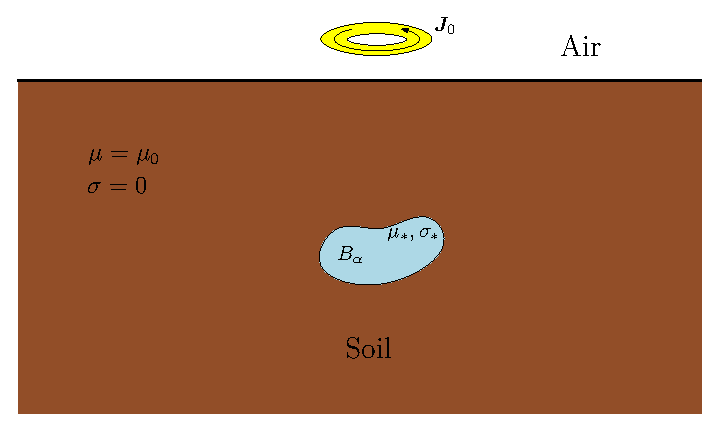
\includegraphics[width=0.7\textwidth, keepaspectratio]{Figures/MetalDetectionSoilSmall.eps}
\caption{A diagram showing a hidden conducting object $B_{\alpha}$ surrounded by it's compliment $B_{\alpha}^c$ which is made up of soil and air.}
\label{metal detection}
\end{center}
\end{figure}
The forward model is described by the system (\ref{Eddy Current}),  which hold in ${\mathbb R}^3$, with
\begin{align}
\mu (\bm{x}) = \left \{  \begin{array}{ll} \mu_* & \bm{x} \in B_{\alpha} \\
\mu_0 & \bm{x} \in B_{\alpha}^c \end{array} \right . ,
\sigma (\bm{x}) = \left \{  \begin{array}{ll} \sigma_* & \bm{x} \in B_{\alpha} \\
0 & \bm{x} \in B_{\alpha}^c \end{array} \right .,
\end{align}
and the regions $B_\alpha$  and $B_\alpha^c $ are coupled by the transmission conditions
\begin{align}
\left [\bm{n} \times \bm{E}_\alpha\right ]_{\Gamma_{\alpha}}=\left [\bm{n} \times \bm{H}_\alpha\right ]_{\Gamma_{\alpha}}=\bm{0},\label{jump}
\end{align}
\noindent
which hold on  $\Gamma_\alpha:= \partial B_\alpha$. In the above, $[u ]_{\Gamma_{\alpha}}:= u| _+ - u|_-  $ denotes the jump,  the $+$ refers to just outside of $B_\alpha$ and the $-$ to just inside and $\bm{n}$ denotes a unit outward normal to  $\Gamma_{\alpha}$. 

The electric interaction field in  (\ref{Eddy Current}) is non-physical and, to ensure uniqueness of this field, the condition $\nabla \cdot \bm{E}_\alpha =0$ is imposed in $B_\alpha^c$. Furthermore,  we also require that $\bm{E}_{\alpha}=O(1/|\bm{x}|)$ and $\bm{H}_{\alpha}=O(1/|\bm{x}|)$  as $|\bm{x} | \to \infty$, denoting that the fields go to zero at least as fast as $1/|\bm{x}|$, although, in practice, this can faster.


\subsubsection{Metal Detection Inverse Problem} \label{sect:inverseproblem}
In the metal detection inverse problem, one wishes to determine the location, shape and material properties of the conducting object $B_\alpha$, described above, from measurements of $(\bm{H}_\alpha - \bm{H}_0) (\bm{x})$ at locations $\bm{x}$ in the air. Here, $\bm{H}_0$ denotes the background magnetic and is the magnetic field that result from the solution of (\ref{Eddy Current}) without the presence of the object $B_\alpha$, i.e.  $\bm{E}_0$ and $\bm{H}_0$ are the solution of (\ref{Eddy Current}) with $\sigma =0$ and $\mu=\mu_0$ in ${\mathbb R}^3$. Similar to above, we also require that $\bm{E}_{0}=O(1/|\bm{x}|)$ and $\bm{H}_{0}=O(1/|\bm{x}|)$  as $|\bm{x} | \to \infty$, denoting that the fields go to zero at least as fast as $1/|\bm{x}|$, although, in practice, this can faster.

Practical metal detectors measure a voltage perturbation, which corresponds to $\int_S \bm{n} \cdot (\bm{H}_\alpha - \bm{H}_0) (\bm{x}) \dif \bm{x}$ over an appropriate surface $S$~\cite{LedgerLionheart2018}. For very small coils, this voltage perturbation corresponds to $\bm{m} \cdot (\bm{H}_\alpha - \bm{H}_0) (\bm{x})$ where $\bm{m}$ is magnetic dipole moment of the coil~\cite{LedgerLionheart2018}.



\subsection{The asymptotic expansion}
The forward problem described in Section~\ref{sect:forward}, implies that if we know $B_\alpha$ ,$ \sigma_*$ and $\mu_*$ we can solve (\ref{Eddy Current})  to determine $\bm{E}_\alpha$ and $\bm{H}_\alpha$. However, to do this repeatably for each new object is computationally expensive. Instead, we seek an approximation in the form of trying approximate the perturbation $(\bm{H}_{\alpha}-\bm{H}_0)( \bm{x})$ at some point $\bm{x}$ exterior to $B_\alpha$.

To do this, following~\cite{Ammari2014,LedgerLionheart2015} we define $B_\alpha := \alpha B + \bm{z}$ where $B$ is a unit size object, $\alpha$ is the object size and $\bm{z}$ is the object's translation from the object as shown in Figure ~\ref{BAlphaShifted}.
\begin{figure}[H]
\begin{center}
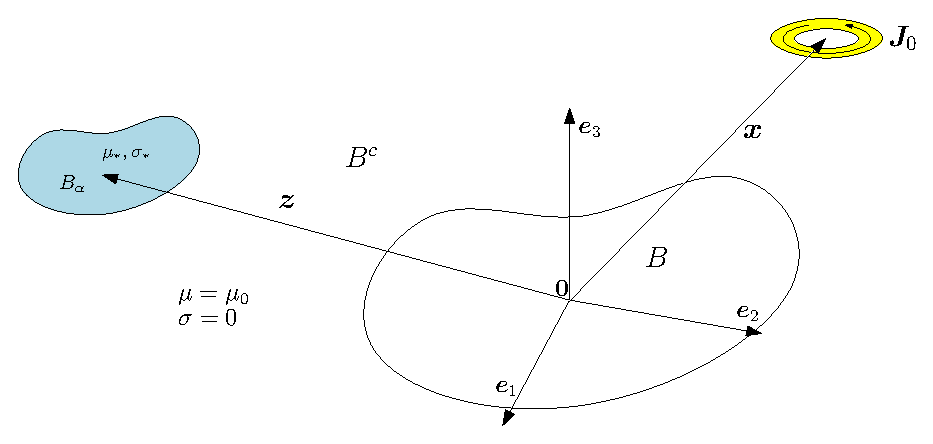
\includegraphics[width=0.8\textwidth, keepaspectratio]{Figures/BAlphaShifted.eps}
\caption{A diagram showing the physical description of $B_{\alpha}$ with respect to the coordinate axes.}
\label{BAlphaShifted}
\end{center}
\end{figure}
\noindent Then, using results obtained by Ammari, Chen, Chen, Garnier and Volkov~\cite{Ammari2014}, Ledger and Lionheart~ \cite{LedgerLionheart2015} have derived the
 asymptotic expansion 
%Asymptotic formula
\begin{align}
(\bm{H}_{\alpha}-\bm{H}_0)(\bm{x})_i=(\bm{D}_{\bm{x}}^2G(\bm{x},\bm{z}))_{ij}(\mathcal{M})_{jk}(\bm{H}_0(\bm{z}))_k+O(\alpha^4), \label{eqn:asymp}
\end{align}
which holds as $\alpha\to 0$. In the above, $G(\bm{x} ,\bm{z}  ) = 1/ {4\pi | \bm{x} -\bm{z} |}$ is the free space Laplace Green's function, $ \bm{D}^2_x G$ denotes the Hessian of $G$ and Einstein summation convention of the indices is implied. The term ${\mathcal M}$ is the symmetric rank 2 magnetic polarizability tensor, which describes the shape and material properties of the object $B_\alpha $ and is independent of the object's position, but is frequency dependent. We will sometimes write $\mathcal{M}[ \alpha B, \omega ]$ to emphasise this. The above formulation, and the definition of ${\mathcal M}$ below, are presented for the case of a single homogenous object $B$, the extension to multiple inhomogeneous objects can be found in~\cite{LedgerLionheartamad2019,LedgerLionheart2019}.

%presented in \cite{LedgerLionheart2015} since it evaluates the object by means of a complex symmetric rank 2 tensor which is invariant relative to position in the field. The expansion also includes an error term, giving a measure of the accuracy of the approximation and is given as follows. We may evaluate the perturbation $(\bm{H}_{\alpha}-\bm{H}_0)$ at the point $\bm{x}$ caused by the object $B_{\alpha}$ as,
%
%which holds as $\alpha\rightarrow 0$. Let us also note the term $\bm{R}(\bm{x})=O(\alpha^4)$ which is the error term we mentioned before. It is also useful for us to note at this point our physical description of $B_{\alpha}$, we define $B_{\alpha}=\alpha B+\bm{z}$ a unit sized object $B$ scaled by $\alpha$ and translated by $\bm{z}$ shown in Figure \ref{BAlphaShifted}.
%B\alpha diagram

\noindent
Let us now turn our attention to the computation of the coefficients of $\mathcal{M}$ in (\ref{eqn:asymp}), which describes the shape and material properties of $B_\alpha$. From the following, will be able compute a library of such tensors for different choices of $\alpha B$ since ${\mathcal M}$ is independent of ${\bm z}$, this, in turn, will lend itself to the application of dictionary based classification algorithms~\cite{LedgerLionheartamad2019} for the solution of the inverse problem stated in Section~\ref{sect:inverseproblem}.


\subsection{Calculating the Magnetic Polarizability Tensor}\label{sectCalculatingMPT}
In the following, we state the explicit formulae for the computation of the coefficients of $\mathcal{M}$, which have been derived in~\cite{LedgerLionheart2019}.  Earlier, Ledger and Lionheart~\cite{LedgerLionheart2015,LedgerLionheart2016,LedgerLionheart2018} have also derived other equivalent formulations, but those below lead to a more natural FEM implementation (using {\texttt{NGSolve}} ).

Following~\cite{LedgerLionheart2019}, we write $\mathcal{M} = ( \mathcal{M})_{ij} \bm{e}_i  \otimes \bm{e}_j$ where $\bm{e}_i$ denotes the $i$th orthonormal unit vector and use the splitting $(\mathcal{M})_{ij}:=(\mathcal{N}^0)_{ij}+(\mathcal{R})_{ij}+\im(  \mathcal{I})_{ij}$ with
%Tensor definitions
\begin{subequations}
\label{eqn:NRI}
\begin{align}
(\mathcal{N}^0[ \alpha B] )_{ij}&:=\alpha^3\delta_{ij}\int_{B}(1-\mu_r^{-1})\dif \bm{\xi}+\frac{\alpha^3}{4}\int_{B\cup B^c}\tilde{\mu}_r^{-1}\nabla\times\tilde{\bm{\theta}}_i^{(0)}\cdot\nabla\times\tilde{\bm{\theta}}_j^{(0)}\ \dif \bm{\xi},\\
(\mathcal{R}[\alpha B, \omega])_{ij}&:=-\frac{\alpha^3}{4}\int_{B\cup B^c}\tilde{\mu}_r^{-1}\nabla\times\bm{\theta}_j^{(1)}\cdot\nabla\times\overline{\bm{\theta}_i^{(1)}}\ \dif \bm{\xi},\\
(\mathcal{I}[\alpha B, \omega])_{ij}&:=\frac{\alpha^3}{4}\int_B\nu\Big(\bm{\theta}_j^{(1)}+(\tilde{\bm{\theta}}_j^{(0)}+\bm{e}_j\times\bm{\xi})\Big)\cdot\Big(\overline{\bm{\theta}_i^{(1)}+(\tilde{\bm{\theta}}_i^{(0)}+\bm{e}_i\times\bm{\xi})}\Big)\ \dif \bm{\xi}.
\end{align}
\end{subequations}
In the above,
\begin{align}
\tilde{\mu}_r ( \bm{\xi} ) := \left \{ \begin{array}{ll}  \mu_r :=\mu_*/\mu_0 & \bm{\xi} \in B\\
1 & \bm{\xi} \in B^c \end{array} \right . \nonumber,
\end{align}
and $\nu:=\alpha^2\omega\mu_0\sigma_*$, $\delta_{ij}$ is the Kronecker delta and the overbar denotes the complex conjugate. The computation of (\ref{eqn:NRI}) rely on the solution of the transmission problems~\cite{LedgerLionheart2019}
\begin{subequations}
\label{eqn:Theta0}
\begin{align}
\nabla\times\tilde{\mu}_r^{-1}\nabla\times\bm{\theta}_i^{(0)}&=\bm{0} &&\textrm{in }B\cup B^c,\\
\nabla\cdot\bm{\theta}_i^{(0)}&=0 &&\textrm{in }B\cup B^c,\\
[{\bm{n}}\times\bm{\theta}_i^{(0)}]_{\Gamma}&=\bm{0} &&\textrm{on }\Gamma,\\
[{\bm{n}}\times\tilde{\mu}_r^{-1}\nabla\times\bm{\theta}_i^{(0)}]_{\Gamma}&=\bm{0} &&\textrm{on }\Gamma,\\
\bm{\theta}_i^{(0)}-{\bm{e}}_i\times\bm{\xi}&=\bm{O}(|\bm{\xi}|^{-1}) &&\textrm{as }|\bm{\xi}|\rightarrow\infty,
\end{align}
\end{subequations}
and 
%Theta 1 transmission problem
\begin{subequations}
\label{eqn:Theta1}
\begin{align}
\nabla\times\mu_r^{-1}\nabla\times\bm{\theta}_i^{(1)}-\im \nu  (\bm{\theta}_i^{(0)}+\bm{\theta}_i^{(1)})&=\bm{0}&&\textrm{in }B,\\
\nabla \times \nabla \times \bm{\theta}_i^{(1)} &= \bm{0} && \text{in }B^c,\\
\nabla\cdot\bm{\theta}_i^{(1)}&=0&&\textrm{in }B^c,\\
[{\bm{n}}\times\bm{\theta}_i^{(1)}]_{\Gamma}&=\bm{0}&&\textrm{on }\Gamma,\\
[{\bm{n}}\times\tilde{\mu}_r^{-1}\nabla\times\bm{\theta}_i^{(1)}]_{\Gamma}&=\bm{0}&&\textrm{on }\Gamma,\\
\bm{\theta}_i^{(1)}(\bm{\xi})&=\bm{O}(|\bm{\xi}|^{-1})&&\textrm{as }|\bm{\xi}|\rightarrow\infty.
\end{align}
\end{subequations}
Note also that $\tilde{\bm{\theta}}_i^{(0)}\vcentcolon=\bm{\theta}_i^{(0)}-\hat{\bm{e}}_i\times\bm{\xi}.$ In order to obtain a discrete approximation using the FEM, we need to introduce a finite computational domain $\Omega$ such that $B\subset\Omega$, whose boundary $\partial\Omega$ is placed sufficiently far from the object $B$. 

The tensor $\mathcal{N}^0[ \alpha B] $ describes the magnetostatic characterisation of $\alpha B$ and is independent of $\omega$. The frequency dependent $\mathcal{R}[\alpha B, \omega]$ tensor vanishes at low frequency and $\mathcal{N}^0[\alpha B]+\mathcal{R}[\alpha B , \omega] =\text{Re}( {\mathcal M} [ \alpha B, \omega]) $ describes the frequency behaviour of the real part of the tensor. Similarly, $\mathcal{I}[\alpha B, \omega] = \text{Im}( {\mathcal M} [ \alpha B, \omega])$ describes the frequency behaviour of the imaginary part of the tensor, which vanishes at low frequencies and  tends to $0$ as the upper limiting frequency of the eddy current model is reached~\cite{LedgerLionheart2019}.

In order to compute the tensor coefficients in (\ref{eqn:NRI}) we need to solve (\ref{eqn:Theta0}) and (\ref{eqn:Theta1}) (repeatably for each $\omega$) and this will be achieved by computing approximate solutions using a range of different numerical schemes
\begin{enumerate}

\item A $hp$ FEM discretisation of the transmission problems (\ref{eqn:Theta0}) and (\ref{eqn:Theta1}) using \texttt{NGSolve}~\cite{NGSolve,zaglmayrphd,netgendet} to compute ${\mathcal M}[\alpha B , \omega]$ for a single frequency.

\item A $hp$ FEM discretisation of the transmission problems (\ref{eqn:Theta0}) and (\ref{eqn:Theta1})  using \texttt{NGSolve}~\cite{NGSolve,zaglmayrphd,netgendet} for performing the  computation of ${\mathcal M}[\alpha B , \omega]$ over a range of frequencies.

\item A  Proper Orthogonal Decomposition (POD) reduced order model, which greatly accelerates the computation of the full order model in 2. for computing ${\mathcal M}[\alpha B , \omega]$ over a range of frequencies.

\item Certificates computed at run time, which indicate the accuracy of the POD outputs with respect to the full order solution over a range of frequencies.



\end{enumerate}

A detailed description of the numerical implementation of these schemes can be found in~\cite{wilsonledger2019}.

In particular, we advocate a $hp$ FEM discretisation using $\bm{H}(\text{curl})$ conforming elements 
for the transmission problems (\ref{eqn:Theta0}) and (\ref{eqn:Theta1}) due to the superior performance it overs over a traditional $h$-version of the FEM, in which only the mesh is refined. In the $hp$-version, the polynomial order of the elements can be increased, as well as refining the finite element grid, in order to obtain accurate solutions. In practice, it is often sufficient to generate a suitable mesh, which has local refinement around sharp edges and corners and increase the polynomial degree in order to obtain accurate solutions for the magnetic polarizability tensor coefficients. As an illustration, we present in Figure~\ref{fig:hprefinement} convergence curves of $\| {\mathcal N}_{hp}^0 - {\mathcal N}^0 \|_F / \| {\mathcal N}^0 \|_F $ and  $\| {\mathcal M}_{hp} - {\mathcal M}\|_F / \| {\mathcal M} \|_F $ computed for a conducting sphere of radius $\alpha=0.01\text{m} $, $\sigma_* =6\times10^6  \text{S/m}$, $\mu_* =1.5 \mu_0$, which has an analytical solution~\cite{Wait1951}, where $hp$ denotes the tensor coefficients obtained by a $hp$ FEM discretisation. The solutions obtained on a sequence of meshes with 12074, 22392, 26751, 48418, 54092, 123788 unstructured tetrahedral elements of order $p=0$ ($h$-refinement) are compared with those obtained on a fixed mesh of 12074 unstructured tetrahedral elements using of order $p=0,1,2,3$, in turn ($p$-refinement). We observe the downward sloping behaviour of the $p$-refinement convergence curve, which illustrates that exponential convergence is being obtained, compared to the slower algebraic rate with $h$-refinement.

\begin{figure}[H]
\begin{center}
$\begin{array}{c}
\includegraphics[width=0.5\textwidth]{GraphsAndData/hp-refinement/N0hp-refinement/N0hp-refinement.pdf} \\
\includegraphics[width=0.5\textwidth]{GraphsAndData/hp-refinement/MPThp-refinement/MPThp-refinement.pdf}
\end{array}$
\caption{Conducting sphere of radius $\alpha=0.01\text{m} $, $\sigma_* = 6\times10^6 \text{S/m}$, $\mu_* =1.5 \mu_0$: Convergence curves of $\| {\mathcal N}_{hp}^0 - {\mathcal N}^0 \|_F / \| {\mathcal N}^0 \|_F $ and  $\| {\mathcal M}_{hp} - {\mathcal M} \|_F / \| {\mathcal M} \|_F $ for $h$ and $p$ refinement}\label{fig:hprefinement}
\end{center}
\end{figure}


 The following describes the installation and use \texttt{MPT-Calculator}, which implements the above schemes.






%%%%%%%%%%%%%%%%%%%%%%%%%%%%%%%%%%%%%%%%%%%%%%%%%%%%%%%%%
%Installing
\section{Installation} \label{sect:install}
Due to the code being written in python and using \texttt{NGSolve} the user is required to install both of these in order to use the \texttt{MPT-Calculator}.  Please follow the instructions available at \href{https://ngsolve.org/}{\texttt{https://ngsolve.org/}} in order to install the high order finite element and meshing library  \texttt{NGSolve}~\cite{NGSolve,zaglmayrphd,netgendet}  released under the LPLG license and ensure a compatible version of Python 3 is installed
%(this varies for different versions of NGSolve and operating systems, although this is documented at \href{https://ngsolve.org/}{\texttt{https://ngsolve.org/}})
which is available at \href{https://www.python.org}{\texttt{https://www.python.org}}. Note that the compatible versions of Python 3 and NGSolve are different on Linux and Mac OS and one should check the NGSolve webpage for up to date information. The code is compatible with \texttt{NGSolve} 6.2.1907 and after. The examples in section \ref{sect:examples} have been run using version 6.2.2004 and version 3.8.2 of \texttt{Python 3}~\cite{python} and meshes for this have also been provided for users runnings different version of NGSolve. The code has been tested on version 10.14.6 of \texttt{MAC OS} and 18.04 of \texttt{Ubuntu}.\\
\\
\noindent
Along with these installations, the \texttt{MPT-Calculator} relies on a number of python packages, which the user is required to install they are as follows \texttt{sys}, \texttt{numpy}, \texttt{os}, \texttt{time}, \texttt{multiprocessing\_on\_dill}, \texttt{cmath}, \texttt{subprocess}, \texttt{matplotlib}. On a MAC or Linux they can be installed from the command line using the command\\
\\
\texttt{pip3 install "package to be installed"}\\
\\
where \texttt{ "package to be installed"} is replaced with the appropriate package name. The user is then required to download or clone the repository of this \texttt{MPT-Calculator} from github. Finally users on Ubuntu are required to enter the following lines into their \texttt{.bashrc} file,\\
\\
\texttt{export OMP\_NUM\_THREADS=1}\\
\texttt{export MKL\_NUM\_THREADS=1}\\
\texttt{export MKL\_THREADING\_LAYER=sequential}\\
\\
This is due to the code calling multiple instances of NGSolve in multiprocessing mode. 





%%%%%%%%%%%%%%%%%%%%%%%%%%%%%%%%%%%%%%%%%%%%%%%%%%%%%%%%%
%Overview of the code
\section{Overview and structure of the code} \label{sect:overview}

Let us now discuss the layout of the code and the files which are designed to be edited. The user is expected interact with 3 files \texttt{main.py}, \texttt{Settings.py} and \texttt{PlotterSettings.py}, these files along with a geometry file (\texttt{.geo} file) (see Section \ref{sect.geo}) allow the user to produce an array of different frequency sweeps for many different objects. In this section we discuss the layout of the folder system in place, how each of the input files can used and edited by the user to produce a frequency sweep along with how and where the results are saved. The structure of the code can be seen in Figure \ref{fig:FrequencySweepCode}
\begin{figure}[H]
\begin{center}
\includegraphics[width=0.4\textwidth]{Figures/CodeLayout}
\caption{Image displaying the structure of the main folder of the FrequencySweepCode.}\label{fig:FrequencySweepCode}
\end{center}
\end{figure}
\noindent
We next discuss how to use the input files of the code.\\
\subsection{User input files}
The files (along with their file paths) the user is expected to interact with are\\
\\
\texttt{main.py}\\
\texttt{Settings/Settings.py}\\
\texttt{Settings/PlotterSettings.py}.\\
\\
Once the files have the desired inputs the simulation is run by entering the command\\
\\
\texttt{python3 main.py}\\
\\
possibly replacing \texttt{python3} with \texttt{python3.8} here and throughout depending on your setup and version installed to the command line from the main directory. The \texttt{MPT-Calculator} then runs the appropriate frequency sweep and saves the outputs in an output folder (see Section \ref{sectOutput}).
We start this explanation with \texttt{main.py}.

\subsubsection{\texttt{main.py}}\label{sectmain.py}
The file \texttt{main.py} is the file with which the user is expected to have most interaction, it is the file which calls functions to generate a mesh, perform frequency sweeps and finally post process the data produced in the frequency sweep. In \texttt{main.py}, the user is greeted with an input section which should look similar to the image in Figure \ref{fig:main.py}.
\begin{figure}[H]
\begin{center}
\includegraphics[width=0.8\textwidth]{Figures/mainpy.pdf}
\caption{Image displaying the user input section of the file \texttt{main.py}}\label{fig:main.py}
\end{center}
\end{figure}
\noindent
In this section we shall briefly explain what each of these inputs refer to and how to provide an input for each. For the first input \texttt{Geometry} the user is required to define the \texttt{.geo} (geometry) file which is to be used in the sweep see Section \ref{sect.geo} for information on how to create geometry files) this input is a string and can be defined as follows \\
\\
\texttt{Geometry = "sphere.geo"}\\
\\
A frequency sweep would then be calculated the object defined in file \texttt{sphere.geo}. The object defined in this file is then scaled by the parameter $\alpha$ (meters), the input for this is a float and can be defined as follows\\
\\
\texttt{alpha = 0.01}\\
\\
This then defines how the object in the \texttt{.geo} file should be scaled. The next two options in the file relate to the mesh which is to be used in the simulation of the object. The variable \texttt{MeshSize} defines how refined the mesh used in the simulation should be, the input for this variable is an integer between 1 and 5 (1 being very coarse and 5 being very fine) and can be defined as follows\\
\\
\texttt{MeshSize = 3}\\
\\
The other key option when it comes to defining a mesh is the order of the elements (how complex the functions describing the solution are) this requires an integer input which is between 0 and 3 (0 being the fastest to run the least accurate and 3 being the slowest by most accurate) when running full simulations (not small tests) it is recommended that an order of 3 be used, this can be defined as follows\\
\\
\texttt{Order = 3}\\
\\
The next 3 inputs relate to the frequencies in radians/sec which should be included in the frequency sweep they are as follows, \texttt{Start} and \texttt{Finish} are the minimum and maximum frequencies which should be included (float) and \texttt{Points} is the number of logarithmically spaced frequencies to be sampled at (integer), n.b. these are the powers base 10 of the frequencies i.e. we create a frequency sweep for $10^{\texttt{Start}}-10^{\texttt{Finish}}$ rad/s. For example if we defined the following\\
\\
\texttt{Start = 1}\\
\texttt{Finish = 8}\\
\texttt{Points = 8}\\
\\
We would run a frequency sweep for 8 logarithmically spaced points between $10^1$ and $10^8$ i.e. for the following frequencies
$$\omega = 10^1,10^2,10^3,10^4,10^5,10^6,10^7,10^8\textrm{ rad/s}.$$
Along with this there is also an option to run a simulation for a single frequency this may be done using the variable \texttt{Single} (boolean) and can be done as follows\\
\\
\texttt{Single $=$ True}\\
\\
This then runs a simulation at the the value defined for the variable \texttt{Omega} (float) n.b. this value is the frequency not the power of 10 of the frequency i.e. setting\\
\\
\texttt{Omega = 133.5}\\
\\
will run a simulation for $\omega=133.5$ rad/s not $\omega=10^{133.5}$ rad/s. If \texttt{Single = False} the frequency sweep will be run for the frequencies defined by \texttt{Start}, \texttt{Finish} and \texttt{Points}. Finally the user will find some options which affect how the frequency sweep will be produced. The first of these is whether or not to create a reduced order model (ROM) using the method of proper orthogonal decomposition (POD) the user may define whether to use this by editing the variable \texttt{POD} (boolean), if the user would like the frequency sweep to be produced using POD they set\\
\\
\texttt{POD = True}\\
\\
The POD works by producing a frequency sweep for a small number of frequencies (snapshots), it then uses the solutions to create an ROM which can then be used to produce a full frequency sweep containing many more points at a fraction of the computational cost. It is useful to note at this point that although POD works very well as the relative permeability $\mu_r$ of the object being simulated increases the POD becomes less accurate, see the spheroid example. This brings us to our final user input in the \texttt{main.py} file which is the variable \texttt{MultiProcessing} this option decides whether to produce the frequency sweep using multiple cores, by setting\\
\\
\texttt{MultiProcessing = True}\\
\\
The wall clock time will be reduced but the frequency sweep then requires more of the machines resources since it is running simulations on multiple cores. The default setting for the number of cores to be used is 2 but can be edited in the default settings section of \texttt{Settings.py}.
\\
\subsubsection{\texttt{Settings/Settings.py}}\label{sectSettings.py}
The second section which the users is able to interact with is the \texttt{Settings.py} file. This file contains settings related to how the frequency sweep is to be run, any addition outputs the user would like, how the data should be saved and how \texttt{NGSolve} solves each of the finite element problems. The file is subdivided into the following sections, \texttt{DefaultSettings}, \texttt{AdditionalOutputs}, \texttt{SaverSettings} and \texttt{SolverParameters}.\\
\\
\\
\noindent
We start by discussing the inputs in \texttt{DefaultSettings}, an image of the section can be seen in Figure \ref{fig:DefaultSettings.py}.
\begin{figure}[H]
\begin{center}
\includegraphics[width=0.7\textwidth]{Figures/DefaultSettings}
\caption{Image displaying the \texttt{DefaultSettings}}\label{fig:DefaultSettings.py}
\end{center}
\end{figure}
\noindent
This section defines variables relating about how to carry out the simulation. The number of cores is set by editing the variable \texttt{CPUs} (integer) an example of this would be setting\\
\\
\texttt{CPUs = 4}\\
\\
which would produce a frequency sweep using 4 of the machines cores. It is useful to mention at this point that when using multiple cores the user is recommended to monitor memory usage especially when producing a frequency sweep for an object with a fine mesh on a machine with limited resources. For larger problems, which are more memory intensive, we have an option for the simulation to use less memory (this option is for POD sweeps only). This is more memory efficient, however, it is both slower and effects performance of both the POD output and POD error bars. This option is engaged by editing the variable \texttt{BigProblem} (boolean), setting\\
\\
\texttt{BigProblem = True}\\
\\
This works by reducing the accuracy and therefore size of the snapshot solutions, saving each complex coefficient using the data type \texttt{np.complex64} (32-bit floats for both the real and imaginary parts). Although the use of this varies for different machines, for reference, using a 2015 mac with 8GB of ram it is advisable to set \texttt{BigProblem = True} for problem larger than 50,000 elements with $p=3$ with 13 snapshots or greater. The next two variables relate to the use of POD the first is \texttt{PODPoints} (integer), this defines how many snapshots should be taken when using the POD method, and can be set as\\
\\
\texttt{PODPoints = 13}\\
\\
This then creates an ROM using 13 snapshots (if \texttt{POD = True} in \texttt{main.py}). The other setting in the the \texttt{DefaultSettings} section is the variable \texttt{PODTol} (float) this variable sets at which point to truncate the singular value decomposition setting\\
\\
\texttt{PODTol = 10**-4}\\
\\
sets the truncation to the point at which the singular values drop below the $10^{-4}$ (for more explanation see~\cite{wilsonledger2019}). Suggested values for \texttt{PODPoints} and \texttt{PODTol} are 13 and $10^{-4}$ respectively. Lastly the setting \texttt{OldMesh} can be used to produce a frequency sweep with a precomputed mesh, saved in a \texttt{.vol} file. Since different versions of NGSolve produce different meshes this option allows you to run new examples using meshes produced on older versions of NGSolce. This is done by specifying the \texttt{.geo} file which contains the material information about the relevant mesh e.g. \texttt{Geometry = myshape.geo}, as well as supplying the \texttt{.vol} file e.g. \texttt{myshape.vol} to the \texttt{VolFiles} folder (this requires the \texttt{.geo} and \texttt{.vol} files to have the same name). Then by setting\\
\\
\texttt{OldMesh = True}\\
\\
the ``old mesh'' is used rather than producing a new mesh.\\
\\
\\
\noindent
Next we will discuss the section \texttt{AdditionalOutputs}, which defines the Additional outputs that the code returns, an image of the section can be seen in Figure \ref{fig:AdditionalOutputs.py}.
\begin{figure}[H]
\begin{center}
\includegraphics[width=0.7\textwidth]{Figures/AdditionalOutputs}
\caption{Image displaying the \texttt{AdditionalOutputs}}\label{fig:AdditionalOutputs.py}
\end{center}
\end{figure}
\noindent
The first variable \texttt{PlotPod} (boolean) defines whether or not to calculate and plot points where the POD has taken snapshots. These points can be plotted by setting\\
\\
\texttt{PlotPod = True}\\
\\
Having these points plotted can be very useful as it gives a visual representation of the accuracy of the frequency sweep produced by POD compared with a full order frequency sweep. We also give the user a way of producing the error certificates by editing the the variable \texttt{PODErrorBars} (boolean) which is selected by setting\\
\\
\texttt{PODErrorBars = True}\\
\\
This then produces error certificates for the POD outputs. The next option \texttt{EddyCurrentTest} (boolean) is to calculate the frequency at which the eddy current model is estimated to break down for the selected object, which may be lower than the prescribed maximum frequency and, for complex objects, may be a considerable restriction. Note this is based on a computation using the object's geometry rather than the standard engineering rules of thumb of saying the object is small compared to the wavelength and the conductivity is high  $\epsilon \omega < \sigma_*$ \cite{schmidt2008estimating}. This is selected by setting\\
\\
\texttt{EddyCurrentTest = True}\\
\\
These three outputs can be produced and saved then chosen to be shown or hidden after the sweep is run. The next two option are for the single frequency solve, with the solution of the single frequency problem the user may export the solution from NGSolve so that it can later be used by programs such as Paraview. This is done by editing the variables \texttt{vtk\_output} (boolean) and \texttt{Refine\_vtk} (boolean), by setting\\
\\
\texttt{vtk\_output = True}\\
\\
a \texttt{.vtk} file will be produced in the \texttt{vtk\_output} section of the \texttt{Results} folder, which contains the eddy-currents in the object. The user may also refine the solution before exporting by setting\\
\\
\texttt{Refine\_vtk = True}\\
\\
It is useful to take note at this point of the size of the files produced by these options an example is of a 2605 element mesh which when exported with no refinement produced a \texttt{.vtk} file of size 956 KB and with refinement produces a \texttt{.vtk} file of size 81.9 MB.\\
\\
\\
\noindent
We next discuss the section \texttt{SaverSettings}, this section allows the user to define a file path within the folder Results to save the outputs of the frequency sweep. An image of the section can be seen in Figure \ref{fig:SaverSettings.py}.
\begin{figure}[H]
\begin{center}
\includegraphics[width=0.7\textwidth]{Figures/SaverSettings}
\caption{Image displaying the \texttt{SaverSettings}}\label{fig:SaverSettings.py}
\end{center}
\end{figure}
\noindent
This is done by changing the variable \texttt{FolderName} (string) to the desired filepath within which save the outputs. An example of this would be\\
\\
\texttt{FolderName = MyShape/MyFrequencySweep}\\
\\
which would then store the output in \texttt{Results/MyShape/MyFrequencySweep}. Although this is an option, we recommend that \texttt{FolderName = "Default"}, which, when set, produces a series of subfolders containing information relating to material properties scaling and frequencies in the sweep. This makes it very hard for the user to overwrite (and lose) existing data from other frequency sweeps, which will be done if the user forgets to change \texttt{FolderName} for a new frequency sweep.\\
\\
\\
\noindent
The final section in \texttt{Settings.py} relates to how \texttt{NGSolve} solves each of the finite element problems. An image of this can be seen in Figure \ref{fig:SolverParameters.py}.
\begin{figure}[H]
\begin{center}
\includegraphics[width=0.7\textwidth]{Figures/SolverParameters}
\caption{Image displaying the \texttt{SolverParameters}}\label{fig:SolverParameters.py}
\end{center}
\end{figure}
\noindent
The default options work well for the frequency sweeps that are presented in the examples section. The default settings are as follows\\
\\
\texttt{Solver = "bddc"}\\
\\
\texttt{epsi = 10**-10}\\
\\
\texttt{Maxsteps = 1500}\\
\\
\texttt{Tolerance = 10**-8}\\
\\
\texttt{ngsglobals.msg\_level = 0}\\
\\
These settings are optimised for meshes containing more than 20,000, $3^{\textrm{rd}}$ order elements, see the examples section for further details. The options for the settings is as follows: The variable \texttt{Solver} (string) can be set to either \texttt{"bddc"} or \texttt{"local"} this changes the preconditioner used by the iterative CG solver in \texttt{NGSolve}. For simulations using very coarse meshes or simulations with $0^{\textrm{th}}$ order elements the \texttt{"local"} preconditioner is faster but for larger simulations setting\\
\\
\texttt{Solver = "bddc"}\\
\\
is recommended. The variable \texttt{tolerance} (float) sets the required relative residual for the iterative CG solver and controls the accuracy of the linear solve. For coarse discretisations, this does not need to be too small. For example, for  full order sweeps, setting\\
\\
\texttt{Tolerance = 10**-6}\\
\\
often leads to satisfactory results, however, upon testing, we found that for the POD the solution needs to be calculated more accurately to capture the underlying behaviour of the solution. The variables \texttt{epsi} (float) (regularisation) and \texttt{Maxsteps} (integer) (the maximum number of iterations performed) are less important since provided that \texttt{epsi} is 1 order of magnitude smaller than \texttt{tolerance} a solution will be reached within the maximum number of iterations. Finally, the variable \texttt{ngsglobals.msg\_level} (integer) relates to the information provided by \texttt{NGSolve} about solving the problems. We recommend that this be set to either \texttt{0} (for no information) or \texttt{3} (for information relating to the assembly and solving of the finite element problems). The next section explains how to use the \texttt{PlotterSettings.py} file.\\
\\
\subsubsection{\texttt{Settings/PlotterSettings.py}}\label{sectPlotterSettings.py}
To display the results of the frequency sweep a simple plotting function has been created\footnote{This is a basic visualisation tool, which allows the user to view results of the sweep. For a graph tailored to the users specification, use the data stored in the \texttt{.csv} files saved in the \texttt{Data} folder to produce their own plot.}, the settings of this function can be edited by changing the inputs of the \texttt{PlotterSettings.py} file. An image of the \texttt{PlotterSettings.py} file can be seen in Figure \ref{fig:PlotterSettings.py}. 
\begin{figure}[H]
\begin{center}
\includegraphics[width=0.8\textwidth]{Figures/PlotterSettingspy}
\caption{Image displaying the file \texttt{PlotterSettings.py}}\label{fig:PlotterSettings.py}
\end{center}
\end{figure}
\noindent
The first two inputs of the file \texttt{EigsToPlot} (list) and \texttt{TensorsToPlot} (list) relate to which lines are to be plotted on the graphs. With these options the user may change both the lines and the order in which the lines are to be plotted. The variable \texttt{EigsToPlot} defines which eigenvalues, sorted smallest to largest, are plotted. For example, setting\\
\\
\texttt{EigsToPlot = [3,2,1]}\\
\\
will plot all of the eigenvalues largest to smallest. The variable \texttt{TensorsToPlot} allows the user to choose which  coefficients of $\mathcal{M}$ are to be plotted. Taking account of the symmetry of the tensor,  the user has a choice of 6 independent coefficients to plot as referenced by the numbers in the following matrix
\begin{align}
\textrm{reference matrix}=\left[\begin{array}{ccc}
1 & 2 & 3\\
2 & 4 & 5\\
3 & 5 & 6
\end{array}\right].
\end{align}
For example, we may plot just diagonal coefficients of the matrix by setting\\
\\
\texttt{TensorsToPlot = [1,4,6]}\\
\\
For simplicity, a legend is created automatically for each of the lines in the plot, without additional inputs required from the user. The next 6 variables relate the style of lines being plotted. The variables \texttt{MainLineStyle} (string), \texttt{SnapshotLineStyle} (string) and \texttt{ErrorBarLineStyle} (string) define the line styles of the full frequency sweep and the line styles of the snapshots and certificate bounds (if \texttt{PlotPod = True} and/ or \texttt{PODErrorBars = True}), respectively. The plots are created using the matplotlib module of python and, thus, the available line styles are those supported by matplotlib \cite{matplotlib}. The other variables relating to line style are \texttt{MainMarkerSize} (float), \texttt{SnapshotMarkerSize} (float) and \texttt{ErrorBarMarkerSize} (float), which define the size of the markers used in the plot for the full sweep, snapshots and certificate bounds, respectively. The recommended settings of these vary on the markers chosen, but the default settings for the line styles and markers are\\
\\
\texttt{MainLineStyle = "-"}
\\
\texttt{MainMarkerSize = 4}
\\
\texttt{SnapshotLineStyle = "x"}
\\
\texttt{SnapshotMarkerSize = 8}
\\
\texttt{ErrorBarLineStyle = "--"}
\\
\texttt{ErrorBarMarkerSize = 4}\\
\\
The next variable, \texttt{EddyCurrentLine} (boolean), defines whether or not to plot the point at which the eddy-current model breaks down. This can be enabled by setting\\
\\
\texttt{EddyCurrentLine = True}\\
\\
The next variable, \texttt{Title} (boolean), defines whether or not the plot includes a title and, again, the title is automatically created for each of the different plots with no user input required. The default setting is\\
\\
\texttt{Title = True}\\
\\
The final variable is \texttt{Show} (boolean), which defines whether or not to display the produced graphs once the frequency sweep is complete\footnote{The graphs are automatically saved this option is whether to display them as well.}. The default setting is\\
\\
\texttt{Show = True}\\
\\
With this we conclude the section on how to interact with each of the input files. We next discuss how and where the output of the code is saved.\\

\subsection{Output files}\label{sectOutput}
In this section, we discuss how the outputs for each of the different versions of the code are saved. As mentioned briefly in Section~\ref{sectSettings.py}, the user may define which folder (or filepath) the outputs are saved in. However, when the code is run, it will generate subfolders to organise the results below this folder (or filepath), as described below. We start with the case of a single frequency simulation.\\


\subsubsection{Single frequency output}
In the case of a simulation with only one frequency, there is no need for a graphical representation, due to this the output folder has the structure shown in Figure \ref{fig:SingleOutput}.
\begin{figure}[H]
\begin{center}
\includegraphics[width=0.3\textwidth]{Figures/SingleOutput}
\caption{Image displaying the structure of the output folder for the case of a single frequency simulation.}\label{fig:SingleOutput}
\end{center}
\end{figure}
\noindent
Notice the inclusion of the folder \texttt{Input\_files}, this folder contains a copy of the inputs files used to run the simulation. This allows the user to reproduce their results, if they so wish. We note the inclusion of the \texttt{sphere.zip} file which is a compressed version of the mesh used for the simulation (\texttt{sphere.vol} file).The folder \texttt{Data}, contains the results for the computed $\mathcal{M}$, $\mathcal{N}^0$, stored in \texttt{MPT.csv} and \texttt{N0.csv}, respectively,  and their eigenvalues $\lambda_i(\mathcal{N}^0+\mathcal{R})$ and $\lambda_i(\mathcal{I})$,  stored in the file \texttt{Eigenvalues.csv} as the sum $\lambda_i(\mathcal{N}^0+\mathcal{R})+\im\lambda_i(\mathcal{I})$ to reduce the number of output files. If the option \texttt{EddyCurrentTest = True} then we also have the \texttt{Eddy-current\_breakdown.txt} file, which states the frequency in rad/s at which the eddy current model breaks down.\\
\\
If the variable \texttt{vtk\_output = True}, we have the added output in the \texttt{vtk\_output} folder of the results folder which can be seen in Figure \ref{fig:VTKOutput}.
\begin{figure}[H]
\begin{center}
\includegraphics[width=0.22\textwidth]{Figures/vtkoutput}
\caption{Image displaying the structure of the output folder for the case of a single frequency simulation.}\label{fig:VTKOutput}
\end{center}
\end{figure}
\noindent
Here we store the \texttt{.vtk} file along with the associated \texttt{.geo} file which contains information about the materials used to construct the object. Let us next discuss the case of a full frequency sweep without using POD.\\

\subsubsection{Full order frequency sweep output}
In the case of the full order frequency sweep, the folder structure for the output folder can be seen in Figure \ref{fig:FullOrderOutput}.

\begin{figure}[H]
\begin{center}
\includegraphics[width=0.35\textwidth]{Figures/FullOutput}
\caption{Image displaying the structure of the output folder for the full order frequency sweep.}\label{fig:FullOrderOutput}
\end{center}
\end{figure}
\noindent
The \texttt{Functions} folder contains the file \texttt{Plotters.py}, which contains the functions used for producing the plots. The folder \texttt{Graphs} contains the graphs displaying the results of the frequency sweep. The file \texttt{Frequencies.csv} contains a list of the frequencies for which the tensors have been calculated and  \texttt{Eigenvalues.csv} contains the sum  $\lambda_i(\mathcal{N}^0+\mathcal{R})+\im\lambda_i(\mathcal{I})$. The file \texttt{Tensors.csv} stores the MPTs coefficient as row vectors and stacks them so that each row corresponds to the same corresponding frequency in the row of the \texttt{Frequencies.csv} file and the eigenvalues in the row of the \texttt{Eigenvalues.csv} file. Finally, the files \texttt{PlotEditor.py} and \texttt{PlotterSettings.py}  allow the user to replot and edit the graphs by editing the inputs in \texttt{PlotterSettings.py} in the same manner as in \ref{sectPlotterSettings.py} and then running the file \texttt{PlotEditor.py}  by entering the command\\

\noindent \texttt{python3 PlotEditor.py}\\
\\
in the command line from the output folder. Next we discuss the case of a frequency sweep produced using POD.\\
\subsubsection{POD frequency sweep output}
In the case of a frequency sweep produced using POD there are two possible options for the structure of the output folder. If \texttt{PlotPod = True}, \texttt{PODErrorBars = True} and \texttt{EddyCurrentTest = True}, the folder will have the structure shown in Figure \ref{fig:PlotPodOutput}.
\begin{figure}[H]
\begin{center}
\includegraphics[width=0.35\textwidth]{Figures/PodOutput}
\caption{Image displaying the structure of the output folder for the frequency sweep using POD with the option of plotting the snapshot tensors.}\label{fig:PlotPodOutput}
\end{center}
\end{figure}
\noindent
The key differences to the full order solve are the inclusion of the data files \texttt{PODFrequencies.csv}, \texttt{PODEigenv\\alues.csv}, \texttt{PODTensors.csv} and \texttt{ErrorBars.csv}. These files contain the frequencies for the snapshots, the eigenvalues of the tensors calculated at the snapshots, the tensors calculated at the snapshots and the certificate bounds of the outputs, respectively. The other difference between this and the full order sweep is the inclusion of the extra plot editor files \texttt{PODPlotEditor.py}, \texttt{PODPlotEditorWithErrorBars.py} and \texttt{PlotEditorWithErrorBars.py}, which enables plots of both the snapshots and full frequency sweep to be reproduced.\\
\\
In the case where \texttt{PlotPod = False},  the structure is as shown in Figure \ref{fig:PlotPodOutput}  except that the files \texttt{PODEigenvalues.csv}, \texttt{PODTensors.csv} and \texttt{PODPlotEditor.py} are not included in the folder. Similarly when \texttt{PODErrorBars = False}, we find the exclusion of the files \texttt{ErrorBars.csv}, \texttt{PODPlotEditorWithError\\Bars.py} and \texttt{PlotEditorWithErrorBars.py} from the output folder. Finally when \texttt{PlotPod  = False} and \texttt{PlotEditorWithErrorBars.py = False} we have the exclusion of \texttt{PODEigenvalues.csv}, \texttt{PODTensors.csv} and \texttt{ErrorBars.csv} along with \texttt{PODPlotEditor.py}, \texttt{PODPlotEditorWithErrorBars.py} and \texttt{PlotEditorWi\\thErrorBars.py}.\\
\\
The user may replot the graphs by entering the commands\\

\noindent \texttt{python3 PlotEditorWithErrorBars.py}\\
\noindent \texttt{python3 PODPlotEditor.py}\\
\noindent \texttt{python3 PODPlotEditorWithErrorBars.py}\\
\\
in the output folder, to show a plot with the snapshots and/ or certificate bounds being displayed on the graph.  Or if the command\\

\noindent \texttt{python3 PlotEditor.py}\\
\\
is entered in the output folder, the graphs without the snapshots included is reproduced. With this we conclude our section on the overview and structure of the code. In the next section, we discuss how to create an object using a \texttt{.geo} file.\\





















 






%%%%%%%%%%%%%%%%%%%%%%%%%%%%%%%%%%%%%%%%%%%%%%%%%%%%%%%%%
%Creating your own geometry file
\section{Creating your own geometry file}\label{sect.geo}

In this section we discuss how to create a geometry file (\texttt{.geo}), with the geometry file being interpreted by \texttt{Netgen}~\cite{netgen} (the meshing tool in \texttt{NGSolve}) we first explain how to create shapes and geometries using a \texttt{.geo} file. \\
\\
Due to \texttt{Netgen} being the underlying interpreter of the \texttt{.geo} file we direct the user to the relevant Constructive Solid Geometry (CSG) documentation available at \href{http://netgen-mesher.sourceforge.net/docs/ng4.pdf}{\texttt{http://netgen-mesher.sourceforge.net/do\\cs/ng4.pdf}}. With this knowledge of this,  we next discuss how the requirements outlined in Section \ref{sectCalculatingMPT}, relating to the  domain $\Omega $, which contains the object $B$, can be specified.
 Finally we explain how to define material properties of the objects being simulated.
\subsection{Truncating the domain}\label{sectTruncating}
Since it is impossible to simulate an infinite computational domain we are required to create a truncated domain $\Omega$ whose boundary $\partial\Omega$ is sufficiently far from the object $B$. In order to do this in the \texttt{.geo} file we simply define a  region which is much larger than the object and place the object at its centre. An example of this is  presented in the \texttt{.geo} file  shown in Figure \ref{fig:ExampleSphere} along with a visualisation of the of the geometry obtained in \texttt{Netgen}.

\begin{figure}[H]
$$\begin{array}{cc}
\includegraphics[width=0.48\textwidth, keepaspectratio]{Figures/ExampleSphere.png} & \includegraphics[width=0.48\textwidth, keepaspectratio]{Figures/ExampleSphereNetgen.png}\\
\textrm{\footnotesize{(a) Example of a \texttt{.geo} file describing a sphere in a sphere}} & \textrm{\footnotesize{(b) Visulisation of the \texttt{.geo} file in (a)}}
\end{array}$$
%\begin{figure}\label{LogvsLin}
\caption{Example of a \texttt{.geo} file (a) describing a sphere of unit radius contained in a domain consisting of a sphere with a radius of 100, with (b) a visualisation of of the constructed geometry using negten.}
\label{fig:ExampleSphere}
\end{figure}
\noindent
This example defines a unit sphere $B$ contained in a domain $\Omega$, which consists of a sphere with a radius of 100. Truncating the domain at a distance approximately 100 times the object size is sufficient for most cases. Next we discuss how to define the material properties of the different regions in the domain.
\subsection{Defining material properties}
To set the material parameters, the user is required to  label each region defined as a Top Level Object (tlo).  This is done by inserting a \texttt{\#} after each toplevel object followed by a label for the material, it's relative permeability $\mu_r$ and it's conductivity $\sigma_*$. We define the material properties for the example presented in the Section \ref{sectTruncating} in  the Figure \ref{fig:ExampleSphereMaterials}.

\begin{figure}[H]
\begin{center}
\includegraphics[width=0.5\textwidth]{Figures/ExampleSphereMaterials.png}
\caption{Image displaying an example of a \texttt{.geo} file with material properties defined for it's regions.}\label{fig:ExampleSphereMaterials}
\end{center}
\end{figure}
\noindent
In Figure \ref{fig:ExampleSphereMaterials}, \texttt{\#sphere -mur=2 -sig=6e+06} labels the object $B$ as \texttt{"sphere"} and defines it's material properties to be $\mu_r=2$ and $\sigma_*=6\times10^6 \text{S/m}$. The inclusion of \texttt{\#air} labels the non conducting region as \texttt{"air"}, which is a protected material and, therefore, does not require the user to input a value for $\mu_r$ or $\sigma_*$. Lastly,  note the inclusion of \texttt{-maxh=0.1} when defining the geometry of $B$. This is an inbuilt function of \texttt{Netgen} for meshing purposes allowing the user to specify a maximum element size for each region in the domain. This is useful since it allows the user to refine the mesh in the conducting region of the domain.\\
\\
Next, we specify the restrictions of the syntax for defining material properties. Any line which starts with \texttt{tlo} (which must have no spaces before) must also contain a material label defined as \texttt{\#material}. On the same line, the user must define both $\mu_r$ and $\sigma_*$ (unless the material is defined to be \texttt{\#air}), to do this the user must provide the flag \texttt{-mur=***} and \texttt{-sig=***} with at least one space between the two flags, but no spaces before or either of the equal signs, and with \texttt{***} replaced with value of the parameter. Note that  $\sigma_*$ should be specified in $\text{S/m}$. Some examples of this can be seen below, first the following examples are accepted,
\begin{align*}
&\texttt{tlo B -col=[1,0,0];\#sphere -mur=2 -sig=6E+06}\\
&\texttt{tlo B -col=[1,0,0];    $\quad$       \#sphere-mur=2 -sig=6E+06}\\
&\texttt{tlo B -col=[1,0,0];\#sphere   $\quad$    -mur=2   $\quad$  -sig=6E+06}
\end{align*}
However, the following examples will not work
\begin{align*}
&\texttt{tlo B -col=[1,0,0];\#sphere -mur = 2 -sig = 6E+06}\\
&\texttt{  tlo B -col=[1,0,0];\#sphere-mur=2 -sig=6E+06}\\
&\texttt{tlo B -col=[1,0,0];\#sphere -mur=2-sig=6E+06}\\
&\texttt{tlo B -col=[1,0,0];\#sphere}\\
&\texttt{-mur=2-sig=6E+06}
\end{align*}
Due to there being a space before or after the equal signs in the first; to a space before the \texttt{tlo} in the second; to the lack of a space between the definition of \texttt{-mur} and \texttt{-sig} in the third and due to the split two lines in the last.
\\
\\
We next consider the case of an object made up of multiple conducting regions follow the examples in Ledger, Lionheart and Amad~\cite{LedgerLionheartamad2019}. We define a conducting rectangular bar, $B$ which is a $2\times1\times1$ block made up 2 distinct sections, contained in a domain bounded by a sphere with radius of 100, as defined in the \texttt{.geo} file shown in Figure \ref{fig:DualBarExample}. Note that $B$ does not have units, the object $\alpha B$ has units with $\alpha$ being the size parameter specified in $\text{m}$ and $\alpha$ is specified later.

\begin{figure}[H]
\begin{center}
\includegraphics[width=0.5\textwidth]{Figures/DualBarExample.png}
\caption{Image displaying an example of a \texttt{.geo} file which defines a bar constructed of 2 regions with different material properties contained in a domain consisting of a sphere with a radius of 100.}\label{fig:DualBarExample}
\end{center}
\end{figure}
\noindent
In Figure \ref{fig:DualBarExample} we have defined two distinct regions \texttt{Block1} and \texttt{Block2} with materials \texttt{"Material1"} and \texttt{"Material2"} having different material properties, respectively.\\
\\
We finish this section with an example of two unit spheres which are constructed using the same material. An example of the \texttt{.geo} file can be seen in Figure \ref{fig:TwoSpheresExample}.

\begin{figure}[H]
\begin{center}
\includegraphics[width=0.5\textwidth]{Figures/TwoSpheresExample.png}
\caption{Image displaying an example of a \texttt{.geo} file which defines a bar constructed of 2 regions with different material properties contained in a domain consisting of a sphere with a radius of 100.}\label{fig:TwoSpheresExample}
\end{center}
\end{figure}
\noindent
This example demonstrates how we only need to define the material properties for \texttt{\#sphere} once even though there are two regions to which it will be applied. This makes it easier to change material properties for a whole geometry when made up of multiple \texttt{tlo}s. We expect this to be useful when working with more complex geometries such as that in the case of a rifle shell, which will be presented in Section \ref{sectRifle}.


\subsection{OCC Geometry}
The current version of \texttt{Netgen} (version 6.2.2203) supports defining object geometries via the Open Cascade Technology (OCC) format. Unlike the \texttt{.geo} file format, the OCC format is purely Python based. I.e. geometries are defined in \texttt{.py} files. Consequently, the user can use standard Python arguments and syntax. For example importing libraries and using iterative loops.\\

\noindent
In the same way as the \texttt{.geo} file format, \texttt{Netgen} constructs complex shapes out of simpler geometric primitives. Currently, \texttt{NGSolve} recommends that OCC geometries be used rather than \texttt{.𝚐𝚎𝚘} files, but there is little documentation available about available primitives and methods. For documentation, we refer the user to the \texttt{NGSolve} documentation and the Open Cascade Technology bottle example:, \href{https://docu.ngsolve.org/latest/i-tutorials/unit-4.4-occ/occ.html?highlight=occ}{here} and \href{https://dev.opencascade.org/doc/overview/html/occt__tutorial.html}{here}.\\

\noindent
An example OCC geometry file to define a unit radius sphere is presented in Listing \ref{lst:OCC_sphere}. In this example we illustrate introducing a unit radius sphere into a larger non-conducting truncated region. This example is included as \texttt{OCC\_Geometry/OCC\_sphere.py}.

\begin{lstlisting}[language=Python, caption={OCC description for a unit radius sphere inside a larger truncated non-conducting region.}, label={lst:OCC_sphere}]
from netgen.occ import *

# Setting mur, sigma, and defining the top level object name:
object_name = 'sphere'
mur = 1
sigma = 1e6

# setting radius
r = 1

# Generating OCC primative sphere centered at [0,0,0] with radius r:
sphere = Sphere(Pnt(0,0,0), r=r)

# Generating surrounding non-conducting region as [-1000,1000]^3 box:
box = Box(Pnt(-1000, -1000, -1000), Pnt(1000,1000,1000))

# setting material and bc names:
# For comparability, we want the non-conducting region to have the 'outer' boundary condition and be labelled as 'air'
sphere.mat(object_name)
sphere.bc('default')
box.mat('air')
box.bc('outer')

# Setting maxh:
sphere.maxh = 0.5
box.maxh = 1000

# Joining the two meshes:
# Glue joins two OCC objects together without interior elemements
joined_object = Glue([sphere, box])

# Generating Mesh:
geo = OCCGeometry(joined_object)
nmesh = geo.GenerateMesh()
nmesh.Save(r'VolFiles/OCC_sphere.vol')
\end{lstlisting}

Similarly to the \texttt{.geo} file format, we make specific mandates for the format. Each OCC geometry file must include:
\begin{lstlisting}[language=Python]
object_name = ['object 1', 'object 2', ... ]
sigma = [conductivity_1, conductivity_2, ...]
mur = [mur_1, mur_2, ...]
\end{lstlisting}
corresponding to the names (string) of the different sub-regions that make up the object and their conductivity (S/m) (float) and relative magnetic permeability (float) values respectively which, in the case of multiple sub-regions can be defined in the form of the lists. In the simplest case, where only one primitive is used, then these can be defined using a single entry. E.g.

\begin{lstlisting}[language=Python]
object_name = 'sphere'
sigma = 1e6
mur = 1
\end{lstlisting}
would define a single object called 'sphere' with conductivity $\sigma_*=10^6$ S/m and relative permeability $\mu_r = 1$.\\

\noindent
In addition, we also mandate that each mesh generated using the OCC format must be save using the same name as the \texttt{.py} file that defines the geometry. For example in Listing \ref{lst:OCC\_sphere}, we have the file name \texttt{OCC\_sphere.py} and save the generated mesh as \texttt{OCC\_sphere.vol}. In a similar way to the \texttt{.geo} file format, each OCC \texttt{.py} file must be stored in the \texttt{OCC\_Geometry} folder and each mesh must be stored in the \texttt{VolFiles} folder.\\

\noindent
Secondly, there must be a valid object description using the available OCC primitives and a defined non-conducting region. For example:
\begin{lstlisting}[language=Python]
sphere = Sphere(Pnt(0,0,0), r=1)
box = Box(Pnt(-1000,-1000,-1000), Pnt(1000,1000,1000))
\end{lstlisting}
defines a sphere of radius 1 and a large cube, centred at (0,0,0) with side length 2000. Note the similarities between the \texttt{.geo} file syntax for a simple primitive and the OCC primitive. We also need to specify material names, boundary condition names, and any additional properties (e.g. \texttt{𝚖𝚊𝚡𝚑}). For compatibility with \texttt{MPT-Calculator}, we want the non-conducting region to have the \texttt{'outer'} boundary condition and be labelled as \texttt{'air'}. In addition, the material name for the conducting object must match one of the entries in \texttt{object\_name}.

\begin{lstlisting}[language=Python]
sphere.mat(object_name[0])
sphere.bc('default')
box.mat('air')
box.bc('outer')
\end{lstlisting}

\noindent
Finally, we need to join the non-conducting region with the conducting object. To avoid interior elements, we use the \texttt{𝙶𝚕𝚞𝚎} method:
\begin{lstlisting}[language=Python]
joined_object = Glue([sphere, box])
\end{lstlisting}
Once the geometric description has been defined, the user must generate and save a mesh. This is done using the \texttt{OCCGeometry}, \texttt{GenerateMesh}, and \texttt{Save} methods. E.g.
\begin{lstlisting}[language=Python]
geo = OCCGeometry(joined_object)
nmesh = geo.GenerateMesh()
nmesh.Save(r'VolFiles/OCC_sphere.vol')
\end{lstlisting}
We recommend that the user maintains a similar style when defining OCC \texttt{.py} files to ensure compatibility. In addition, \texttt{GenerateMesh} admits multiple meshing arguments, such as \texttt{meshsize.very\_coarse}, \texttt{meshsize.coarse}, \texttt{meshsize.moderate}, ect that have the same effect as the mesh size options discussed in Section~\ref{sectmain.py}.\\

\noindent
Further examples are provided in the \texttt{OCC\_Geometry} folder.





%%%%%%%%%%%%%%%%%%%%%%%%%%%%%%%%%%%%%%%%%%%%%%%%%%%%%%%%%
%Examples
\section{Examples} \label{sect:examples}
In this section, we consider a set of examples in which the functionality of the \texttt{MPT-Calculator} is demonstrated. Note that these examples have been run with NGSolve 6.2.2004 if running with a different versions the user may obtain different meshes, due to this the meshes used to produce the results have been included in the VolFiles folder. We start with the case of a sphere.
\subsection{Sphere}\label{sectSphereSweeps}
For the case where $B$ is a sphere of unit radius and $\alpha B$ is a sphere of radius $\alpha=0.01 \text{m}$ we shall create three different simulations, the first is a simulation consisting of a single frequency, the second a full order frequency sweep and the third a frequency sweep implementing the POD. All of these sphere examples are created using the \texttt{sphere.geo} file, shown in Figure \ref{fig:SweepSphere}, where $\Omega$ is chosen to be a ball of radius 200 containing the object $B$, $\sigma_*=6\times 10^6\text{ S/m}$ and $\mu_*=1.5\mu_0$.
\begin{figure}[H]
\begin{center}
\includegraphics[width=0.5\textwidth]{Figures/SweepSphere.png}
\caption{Image displaying the \texttt{Sphere.geo} file used in all of the sphere frequency sweep examples in Section \ref{sectSphereSweeps}.}\label{fig:SweepSphere}
\end{center}
\end{figure}
\noindent
We start our examples session with a simulation of the sphere described in Figure \ref{fig:SweepSphere} for a single frequency.
\subsubsection{Single frequency sweep for a sphere}
To set up this simulation, we used the \texttt{sphere.geo} file shown in Figure \ref{fig:SweepSphere} along with the inputs displayed in Figure \ref{fig:SphereSingleInputs}.
\begin{figure}[H]
$$\begin{array}{ccc}
\includegraphics[width=0.3\textwidth, keepaspectratio]{Figures/SphereMain} & \includegraphics[width=0.3\textwidth, keepaspectratio]{Figures/SphereSettingsTop} & \includegraphics[width=0.3\textwidth, keepaspectratio]{Figures/SphereSettingsBottom}\\
\textrm{\footnotesize{(a) An image of \texttt{main.py}.}} & \textrm{\footnotesize{(b) Top of \texttt{Settings.py}.}} & \textrm{\footnotesize{(c) Bottom of \texttt{Settings.py}.}}
\end{array}$$
%\begin{figure}\label{LogvsLin}
\caption{Images displaying the inputs for the single frequency sweep for a sphere (a) image of the inputs in \texttt{main.py} (b) image of the inputs in the top of \texttt{Settings.py} (c) image of the inputs in the bottom of \texttt{Settings.py}.}
\label{fig:SphereSingleInputs}
\end{figure}
\noindent
These inputs for \texttt{main.py} and \texttt{Settings.py} have been summarised in Table \ref{tab:SphereSingleInputs}. As  \texttt{Single = True} the following variables are not used: \texttt{Start = 1}, \texttt{Finish = 8}, \texttt{Points = 81}, \texttt{Pod = False}, \texttt{PODPoints = 13}, \texttt{PODTol = 10**-4}, \texttt{PlotPod = False} and \texttt{PODErrorBars = False}, hence, their values are arbitrary. 
%\begin{table}[H]
%\begin{center}
%\begin{tabular}{!\vrule l!\vrule l!\vrule l!\vrule}
%\hline
%\texttt{Geometry = "sphere.geo"} & \texttt{Pod = False} & \texttt{EddyCurrentTest = False}\\\hline
%\texttt{alpha = 0.01} & \texttt{MultiProcessing = True} & \texttt{vtk\_output = False}\\\hline
%\texttt{MeshSize = 2} & \texttt{CPUs = 3} & \texttt{Refine\_vtk = False}\\\hline
%\texttt{Order = 3} & \texttt{BigProblem = False} & \texttt{FolderName = "Default"}\\\hline
%\texttt{Start = 1} & \texttt{PODPoint = 13} & \texttt{Solver = "bddc"}\\\hline
%\texttt{Finish = 8} & \texttt{PODTol = 10**-4} & \texttt{epsi = 10**-10}\\\hline
%\texttt{Points = 81} & \texttt{OldMesh = False} & \texttt{Maxsteps = 1500}\\\hline
%\texttt{Single = True} & \texttt{PlotPod = False} & \texttt{Tolerance = 10**-8}\\\hline
%\texttt{Omega = 133.5} & \texttt{PODErrorBars = False} & \texttt{ngsglobals.msg\_level = 0}\\\hline
%\end{tabular}
\begin{table}[H]
\begin{center}
\large{\texttt{main.py}}\normalsize{ }\\\vspace{0.2cm}
\begin{tabular}{!\vrule p{4.5cm}!\vrule p{4.5cm}!\vrule p{4.5cm}!\vrule}
\hline
\texttt{Geometry = "sphere.geo"} & \texttt{alpha = 0.01} & \texttt{MeshSize = 2}\\\hline
\texttt{Order = 3} & \texttt{Start = 1} & \texttt{Finish = 8}\\\hline
\texttt{Points = 81} & \texttt{Single = True} &\texttt{Omega = 133.5}\\\hline
\end{tabular}\\
\begin{tabular}{!\vrule p{4.5cm}!\vrule p{4.5cm}!\vrule}
\texttt{Pod = False} & \texttt{MultiProcessing = True}\\\hline
\end{tabular}
\\\vspace{0.5cm}\large{\texttt{Settings.py}}\normalsize{ }\\\vspace{0.2cm}
\begin{tabular}{!\vrule p{4.5cm}!\vrule p{4.5cm}!\vrule p{4.5cm}!\vrule}
\hline
\texttt{CPUs = 3} & \texttt{BigProblem = False} & \texttt{PODPoints = 13}\\\hline
\texttt{PODTol = 0.0001} & \texttt{OldMesh = False} & \texttt{PlotPod = False}\\\hline
\texttt{PODErrorBars = False} & \texttt{EddyCurrentTest = False} & \texttt{vtk\_output = False}\\\hline
\texttt{Refine\_vtk = False} & \texttt{FolderName = "Default"} & \texttt{Solver = "bddc"}\\\hline
\texttt{epsi = 1e-10} & \texttt{Maxsteps = 1500} & \texttt{Tolerance = 1e-08}\\\hline
\end{tabular}\\
\begin{tabular}{!\vrule p{4.5cm}!\vrule}
\texttt{ngsglobals.msg\_level = 0}\\\hline
\end{tabular}\caption{A table summarising the inputs for the simulation of the sphere with for a single frequency.}\label{tab:SphereSingleInputs}
\end{center}
\end{table}
\noindent
This means our interest lies in computing the characterisation for $ \alpha B = 0.01 B$ at a frequency of $\omega = 133.5 \text{rad/s}$.
Furthermore, the inputs led to a mesh of 29170 elements and a discretisation of $p=3$. On a 2012 iMac with a 2.9 GHz quad core i5 processor with 16 GB 1600 MHz DDR3 memory the computation takes 1 minute and 37 seconds using $3$ CPUs and results in the following for the $\mathcal{N}^0$ and $\mathcal{M}$,
\begin{align*}
\mathcal{N}_{hp}^0 = \left(\begin{array}{ccc}
1.80\times10^{-6} & 6.06\times10^{-14} & 1.89\times10^{-15}\\
6.06\times10^{-14} & 1.80\times10^{-6} & 9.55\times10^{-14}\\
1.89\times10^{-15} & 9.55\times10^{-14} & 1.80\times10^{-6}
\end{array}\right),
\end{align*}
\begin{align*}
\mathcal{M}_{hp} = \left(\begin{array}{ccc}
1.79\times10^{-6}+6.97\times10^{-8}\rm{i} & 5.85\times10^{-14}+6.61\times10^{-15}\rm{i} & -3.53\times10^{-15}+2.23\times10^{-14}\rm{i}\\
5.85\times10^{-14}+6.61\times10^{-15}\rm{i} & 1.79\times10^{-6}+6.97\times10^{-8}\rm{i} & 9.06\times10^{-14}+3.18\times10^{-14}\rm{i}\\
-3.53\times10^{-15}+2.23\times10^{-14}\rm{i} & 9.06\times10^{-14}+3.18\times10^{-14}\rm{i} & 1.79\times10^{-6}+6.97\times10^{-8}\rm{i}
\end{array}\right).
\end{align*}
The exact tensors for this object are known to be diagonal and multiple of identity~\cite{LedgerLionheart2018,Wait1951}. Specifically $(\mathcal{N})_{ii} = 1.80 \times 10^{-6} $ and $(\mathcal{M})_{ii} =  1.79 \times 10^{-6} +6.97 \times 10^{-8} \im $ to 2dp. By repeatably performing $h$ or $p$ refinement, the off diagonal terms tend to $0$ and the diagonal entries of $\mathcal{M}_{hp}$ and  $\mathcal{N}_{hp}$ to their exact values according to the convergence curves presented in Figure \ref{fig:hprefinement}. In this case, the relative error $\| \mathcal{M}- \mathcal{M}_{hp} \|_F / \|\mathcal{M}  \|_F = 2.72 \times 10^{-6}$. We also find the computed eigenvalues to be
\begin{align*}
\lambda(\mathcal{N}^0+\mathcal{R}) = \left(\begin{array}{c}
1.79\times10^{-6}\\1.79\times10^{-6}\\1.79\times10^{-6}
\end{array}\right),\quad
\lambda(\mathcal{I}) = \left(\begin{array}{c}
6.97\times10^{-8}\\6.97\times10^{-8}\\6.97\times10^{-8}
\end{array}\right).
\end{align*}
We next consider the example of a full order frequency sweep once again for the sphere described by the \texttt{.geo} file in Figure \ref{fig:SweepSphere}.
\subsubsection{Full order frequency sweep for a sphere}
A frequency sweep is now performed for the sphere described by the \texttt{sphere.geo} file in Figure \ref{fig:SweepSphere} along with the inputs represented in Table \ref{tab:SphereFullInputs}. As  \texttt{Single = False} and \texttt{Pod = False} the following variables are not used \texttt{Omega = 133.5}, \texttt{PODPoints = 13}, \texttt{PODTol = 10**-4} and \texttt{PODErrorBars = False}, hence, their values are arbitrary.
%\begin{table}[H]
%\begin{center}
%\begin{tabular}{!\vrule l!\vrule l!\vrule l!\vrule}
%\hline
%\texttt{Geometry = "sphere.geo"} & \texttt{Pod = False} & \texttt{EddyCurrentTest = False}\\\hline
%\texttt{alpha = 0.01} & \texttt{MultiProcessing = True} & \texttt{vtk\_output = False}\\\hline
%\texttt{MeshSize = 2} & \texttt{CPUs = 4} & \texttt{Refine\_vtk = False}\\\hline
%\texttt{Order = 3} & \texttt{BigProblem = False} & \texttt{FolderName = "Default"}\\\hline
%\texttt{Start = 1} & \texttt{PODPoints = 13} & \texttt{Solver = "bddc"}\\\hline
%\texttt{Finish = 8} & \texttt{PODTol = 0.0001} & \texttt{epsi = 1e-10}\\\hline
%\texttt{Points = 81} & \texttt{OldMesh = False} & \texttt{Maxsteps = 1500}\\\hline
%\texttt{Single = False} & \texttt{PlotPod = False} & \texttt{Tolerance = 1e-08}\\\hline
%\texttt{Omega = 133.5} & \texttt{PODErrorBars = False} & \texttt{ngsglobals.msg\_level = 0}\\\hline
%\end{tabular}
\begin{table}[H]
\begin{center}
\large{\texttt{main.py}}\normalsize{ }\\\vspace{0.2cm}
\begin{tabular}{!\vrule p{4.5cm}!\vrule p{4.5cm}!\vrule p{4.5cm}!\vrule}
\hline
\texttt{Geometry = "sphere.geo"} & \texttt{alpha = 0.01} & \texttt{MeshSize = 2}\\\hline
\texttt{Order = 3} & \texttt{Start = 1} & \texttt{Finish = 8}\\\hline
\texttt{Points = 81} & \texttt{Single = False} &\texttt{Omega = 133.5}\\\hline
\end{tabular}\\
\begin{tabular}{!\vrule p{4.5cm}!\vrule p{4.5cm}!\vrule}
\texttt{Pod = False} & \texttt{MultiProcessing = True}\\\hline
\end{tabular}
\\\vspace{0.5cm}\large{\texttt{Settings.py}}\normalsize{ }\\\vspace{0.2cm}
\begin{tabular}{!\vrule p{4.5cm}!\vrule p{4.5cm}!\vrule p{4.5cm}!\vrule}
\hline
\texttt{CPUs = 4} & \texttt{BigProblem = False} & \texttt{PODPoints = 13}\\\hline
\texttt{PODTol = 0.0001} & \texttt{OldMesh = False} & \texttt{PlotPod = False}\\\hline
\texttt{PODErrorBars = False} & \texttt{EddyCurrentTest = False} & \texttt{vtk\_output = False}\\\hline
\texttt{Refine\_vtk = False} & \texttt{FolderName = "Default"} & \texttt{Solver = "bddc"}\\\hline
\texttt{epsi = 1e-10} & \texttt{Maxsteps = 1500} & \texttt{Tolerance = 1e-08}\\\hline
\end{tabular}\\
\begin{tabular}{!\vrule p{4.5cm}!\vrule}
\texttt{ngsglobals.msg\_level = 0}\\\hline
\end{tabular}
\caption{A table summarising the inputs for the simulation of a sphere for a full order frequency sweep.}\label{tab:SphereFullInputs}
\end{center}
\end{table}
\noindent
This means our interest lies in computing the characterisation for $\alpha B = 0.01 B$ at 81 frequencies in the range $10^1\leq\omega\leq10^8\text{rad/s}$. Furthermore, the inputs lead to a mesh of 29170 elements and a discretisation of $p=3$. On a 2012 iMac with a 2.9 GHz quad core i5 processor with 16 GB 1600 MHz DDR3 memory the computation takes 1 hour 2 minutes 44 seconds using $4$ CPUs, from this we obtain the results shown in Figure \ref{fig:FullOrderSphere}.
\begin{figure}[H]
$$\begin{array}{cc}
\includegraphics[width=0.48\textwidth, keepaspectratio]{Figures/FullExactReal/FullExactReal.pdf} & \includegraphics[width=0.48\textwidth, keepaspectratio]{Figures/FullExactImag/FullExactImag.pdf}\\
\textrm{\footnotesize{(a) A graph showing how $\lambda_1(\mathcal{N}^0+\mathcal{R})$ changes with frequency.}} & \textrm{\footnotesize{(b) A graph showing how $\lambda_1(\mathcal{I})$ changes with frequency.}}
\end{array}$$
%\begin{figure}\label{LogvsLin}
\caption{Graphs displaying the eigenvalues of both the real and imaginary parts for $\mathcal{M}$ calculated using a full order frequency sweep for a sphere compared with the exact values.}
\label{fig:FullOrderSphere}
\end{figure}
\noindent
In Figure \ref{fig:FullOrderSphere}, we only show the first eigenvalues $\lambda_1({\mathcal R}+{\mathcal N}^0)$ and $\lambda_1({\mathcal I})$, this is due to the difference between $\lambda_1,\lambda_2,\lambda_3$ being negligible in each case. We also show the exact values of the eigenvalues, which corresponds to the diagonal coefficients of the tensors in this case~\cite{LedgerLionheart2018,Wait1951}, in order to illustrate the performance of the sweep. Note that the code does not produce the exact value for  $\lambda_1({\mathcal R}+{\mathcal N}^0)$ and $\lambda_1({\mathcal I})$ and these have been included afterwards for demonstration purposes. From a visual inspection, the simulation has obtained very good results and this is confirmed by a sweep of  the relative error shown in Figure \ref{fig:FullOrderSphereError}, which shows the maximum relative error is 0.006 over the  sweep.
\begin{figure}[H]
\begin{center}
\includegraphics[width=0.5\textwidth]{Figures/FullError/FullError.pdf}
\caption{A graph showing how the relative error in the first eigenvalue changes due to frequency.}\label{fig:FullOrderSphereError}
\end{center}
\end{figure}
\noindent
We next consider the case of a the reduced order frequency sweep using the POD.
\subsubsection{POD frequency sweep for a sphere}
For this frequency sweep , the sphere described by the \texttt{sphere.geo} file in Figure \ref{fig:SweepSphere} is simulated with the inputs as shown in Table \ref{tab:SpherePODInputs}. As  \texttt{Single = False} the following variables are not used:  \texttt{Omega = 133.5}  hence their values are arbitrary.
%\begin{table}[H]
%\begin{center}
%\begin{tabular}{!\vrule l!\vrule l!\vrule l!\vrule}
%\hline
%\texttt{Geometry = "sphere.geo"} & \texttt{Pod = True} & \texttt{EddyCurrentTest = False}\\\hline
%\texttt{alpha = 0.01} & \texttt{MultiProcessing = True} & \texttt{vtk\_output = False}\\\hline
%\texttt{MeshSize = 2} & \texttt{CPUs = 4} & \texttt{Refine\_vtk = False}\\\hline
%\texttt{Order = 3} & \texttt{BigProblem = False} & \texttt{FolderName = "Default"}\\\hline
%\texttt{Start = 1} & \texttt{PODPoints = 13} & \texttt{Solver = "bddc"}\\\hline
%\texttt{Finish = 8} & \texttt{PODTol = 0.0001} & \texttt{epsi = 1e-10}\\\hline
%\texttt{Points = 81} & \texttt{OldMesh = False} & \texttt{Maxsteps = 1500}\\\hline
%\texttt{Single = False} & \texttt{PlotPod = True} & \texttt{Tolerance = 1e-08}\\\hline
%\texttt{Omega = 133.5} & \texttt{PODErrorBars = False} & \texttt{ngsglobals.msg\_level = 0}\\\hline
%\end{tabular}
\begin{table}[H]
\begin{center}
\large{\texttt{main.py}}\normalsize{ }\\\vspace{0.2cm}
\begin{tabular}{!\vrule p{4.5cm}!\vrule p{4.5cm}!\vrule p{4.5cm}!\vrule}
\hline
\texttt{Geometry = "sphere.geo"} & \texttt{alpha = 0.01} & \texttt{MeshSize = 2}\\\hline
\texttt{Order = 3} & \texttt{Start = 1} & \texttt{Finish = 8}\\\hline
\texttt{Points = 81} & \texttt{Single = False} &\texttt{Omega = 133.5}\\\hline
\end{tabular}\\
\begin{tabular}{!\vrule p{4.5cm}!\vrule p{4.5cm}!\vrule}
\texttt{Pod = True} & \texttt{MultiProcessing = True}\\\hline
\end{tabular}
\\\vspace{0.5cm}\large{\texttt{Settings.py}}\normalsize{ }\\\vspace{0.2cm}
\begin{tabular}{!\vrule p{4.5cm}!\vrule p{4.5cm}!\vrule p{4.5cm}!\vrule}
\hline
\texttt{CPUs = 4} & \texttt{BigProblem = False} & \texttt{PODPoints = 13}\\\hline
\texttt{PODTol = 0.0001} & \texttt{OldMesh = False} & \texttt{PlotPod = True}\\\hline
\texttt{PODErrorBars = False} & \texttt{EddyCurrentTest = False} & \texttt{vtk\_output = False}\\\hline
\texttt{Refine\_vtk = False} & \texttt{FolderName = "Default"} & \texttt{Solver = "bddc"}\\\hline
\texttt{epsi = 1e-10} & \texttt{Maxsteps = 1500} & \texttt{Tolerance = 1e-08}\\\hline
\end{tabular}\\
\begin{tabular}{!\vrule p{4.5cm}!\vrule}
\texttt{ngsglobals.msg\_level = 0}\\\hline
\end{tabular}
\caption{A table summarising the inputs for the simulation of a sphere for a reduced order frequency sweep.}\label{tab:SpherePODInputs}
\end{center}
\end{table}
\noindent
This means our interest lies in computing the characterisation for $\alpha B=0.01 B$ at 81 output frequencies in the range $10^1\leq\omega\leq10^8\text{rad/s}$ using  the same mesh of 29170 elements and a $p=3$ discretisation. However, the result is now generated by using a POD technique in which  $13$ snapshots are chosen logarithmically (following the approach described in Section \ref{sectmain.py}) in order to create to create the ROM. On a 2012 iMac with a 2.9 GHz quad core i5 processor with 16 GB 1600 MHz DDR3 memory the computation took 12 minutes and 28 seconds using $4$ CPUs leading to the results shown in Figure \ref{fig:PODSphere}\footnote{The POD frequency sweep in Figure \ref{fig:PODSphere} has been produced with \texttt{ImagTensorFullOrderCalc = True} see Section \ref{Issues} for more details.}.
\begin{figure}[H]
$$\begin{array}{cc}
\includegraphics[width=0.48\textwidth, keepaspectratio]{Figures/PODExactReal/PODExactReal.pdf} & \includegraphics[width=0.48\textwidth, keepaspectratio]{Figures/PODExactImag/PODExactImag.pdf}\\
\textrm{\footnotesize{(a) A graph showing how $\lambda_1(\mathcal{N}^0+\mathcal{R})$ changes with frequency.}} & \textrm{\footnotesize{(b) A graph showing how $\lambda_1(\mathcal{I})$ changes with frequency.}}
\end{array}$$
%\begin{figure}\label{LogvsLin}
\caption{Graphs displaying the eigenvalues of both the real and imaginary parts for $\mathcal{M}$ calculated using a frequency sweep which implemented a POD for a sphere compared with the exact values.}
\label{fig:PODSphere}
\end{figure}
\noindent
Again only the first eigenvalues $\lambda_1({\mathcal R}+{\mathcal N}^0)$ and $\lambda_1({\mathcal I})$ are shown  together with their exact values, added in a post-processing step. From Figure \ref{fig:PODSphere}, we see that the sweep is very accurate and this is confirmed by showing the relative error as a function of frequency  in Figure \ref{fig:PODSphereError}.
\begin{figure}[H]
\begin{center}
\includegraphics[width=0.5\textwidth]{Figures/PODError/PODError.pdf}
\caption{A graph showing how the relative error in the first eigenvalue changes due to frequency.}\label{fig:PODSphereError}
\end{center}
\end{figure}
\noindent
From Figure \ref{fig:PODSphereError}, we see that the performance is good, if not better, than the full order model, but only requires $13$ full order model snapshots
and took a quarter of the time of the full order model. However, if we set \texttt{PODErrorBars =True} then we obtain upper bounds on the difference between the full order and POD frequency sweeps. An example of this can be seen in Figure \ref{fig:PODSphereErrorBars} this was run for 21 snapshots with a POD tolerance of $10^{-6}$. Note that these certificate bounds are computed at run time with minimal additional computational cost. For further details of the cost break down and additional examples of certificate bounds see \cite{wilsonledger2019}.
\begin{figure}[H]
$$\begin{array}{cc}
\includegraphics[width=0.48\textwidth, keepaspectratio]{Figures/SphereErrorBarsRealn=21.pdf} & \includegraphics[width=0.48\textwidth, keepaspectratio]{Figures/SphereErrorBarsImagn=21.pdf}\\
\textrm{\footnotesize{(a) A graph showing how $(\mathcal{N}^0+\mathcal{R})_{11}$ changes with frequency.}} & \textrm{\footnotesize{(b) A graph showing how $(\mathcal{I})_{11}$ changes with frequency.}}
\end{array}$$
\caption{A graph showing the certificate bounds produced for the sphere with 21 snapshots with a POD tolerance of $10^{-6}$.}\label{fig:PODSphereErrorBars}
\end{figure}
\noindent
For more detail about how the bounds are computed along with other examples please see \cite{wilsonledger2019}. With this we conclude the examples of the sphere, we next consider a simulation of a conducting permeable torus.
\subsection{Torus}
In this section, we consider the case where $B$  is a torus with a major and minor radii of  of 2 and  1, respectively, and the physical object $\alpha B$ is created from this object using the scaling $\alpha=0.01\text{m}$. We simulate a full order frequency sweep using the \texttt{Torus.geo} file shown in Figure \ref{fig:torus.geo}, where $\Omega$ is chosen to be a ball of radius 100 containing the object $B$ with material parameters $\sigma_*=5.96\times10^6\text{ S/m}$ and $\mu_*=1.5\mu_0$.
\begin{figure}[H]
\begin{center}
\includegraphics[width=0.5\textwidth]{Figures/TorusInput.png}
\caption{An image showing the \texttt{Torus.geo} file used to simulate the torus.}\label{fig:torus.geo}
\end{center}
\end{figure}
\noindent
To set up this simulation, we used the \texttt{Torus.geo} file shown in Figure \ref{fig:torus.geo} along with the inputs summarised in Table \ref{tab:TorusInputs}.
%\begin{table}[H]
%\begin{center}
%\begin{tabular}{!\vrule l!\vrule l!\vrule l!\vrule}
%\hline
%\texttt{Geometry = "Torus.geo"} & \texttt{Pod = False} & \texttt{EddyCurrentTest = False}\\\hline
%\texttt{alpha = 0.01} & \texttt{MultiProcessing = True} & \texttt{vtk\_output = False}\\\hline
%\texttt{MeshSize = 3} & \texttt{CPUs = 4} & \texttt{Refine\_vtk = False}\\\hline
%\texttt{Order = 3} & \texttt{BigProblem = False} & \texttt{FolderName = "Default"}\\\hline
%\texttt{Start = 1} & \texttt{PODPoints = 13} & \texttt{Solver = "bddc"}\\\hline
%\texttt{Finish = 8} & \texttt{PODTol = 0.0001} & \texttt{epsi = 1e-10}\\\hline
%\texttt{Points = 81} & \texttt{OldMesh = False} & \texttt{Maxsteps = 1500}\\\hline
%\texttt{Single = False} & \texttt{PlotPod = True} & \texttt{Tolerance = 1e-08}\\\hline
%\texttt{Omega = 133.5} & \texttt{PODErrorBars = False} & \texttt{ngsglobals.msg\_level = 0}\\\hline
%\end{tabular}
\begin{table}[H]
\begin{center}
\large{\texttt{main.py}}\normalsize{ }\\\vspace{0.2cm}
\begin{tabular}{!\vrule p{4.5cm}!\vrule p{4.5cm}!\vrule p{4.5cm}!\vrule}
\hline
\texttt{Geometry = "Torus.geo"} & \texttt{alpha = 0.01} & \texttt{MeshSize = 3}\\\hline
\texttt{Order = 3} & \texttt{Start = 1} & \texttt{Finish = 8}\\\hline
\texttt{Points = 81} & \texttt{Single = False} &\texttt{Omega = 133.5}\\\hline
\end{tabular}\\
\begin{tabular}{!\vrule p{4.5cm}!\vrule p{4.5cm}!\vrule}
\texttt{Pod = False} & \texttt{MultiProcessing = True}\\\hline
\end{tabular}
\\\vspace{0.5cm}\large{\texttt{Settings.py}}\normalsize{ }\\\vspace{0.2cm}
\begin{tabular}{!\vrule p{4.5cm}!\vrule p{4.5cm}!\vrule p{4.5cm}!\vrule}
\hline
\texttt{CPUs = 4} & \texttt{BigProblem = False} & \texttt{PODPoints = 13}\\\hline
\texttt{PODTol = 0.0001} & \texttt{OldMesh = False} & \texttt{PlotPod = True}\\\hline
\texttt{PODErrorBars = False} & \texttt{EddyCurrentTest = False} & \texttt{vtk\_output = False}\\\hline
\texttt{Refine\_vtk = False} & \texttt{FolderName = "Default"} & \texttt{Solver = "bddc"}\\\hline
\texttt{epsi = 1e-10} & \texttt{Maxsteps = 1500} & \texttt{Tolerance = 1e-08}\\\hline
\end{tabular}\\
\begin{tabular}{!\vrule p{4.5cm}!\vrule}
\texttt{ngsglobals.msg\_level = 0}\\\hline
\end{tabular}
\caption{A table summarising the inputs for the simulation of a torus for a reduced order frequency sweep.}
\label{tab:TorusInputs}
\end{center}
\end{table}
\noindent
This means our interest lies in computing the characterisation for $\alpha B=0.01B$ at 81 frequencies in the range $10^1\leq\omega\leq10^8\text{ rad/s}$. Furthermore, the inputs lead to a mesh of 32008 elements and a discretisation of $p=3$. On a 2012 iMac with a 2.9 GHz quad core i5 processor with 16 GB 1600 MHz DDR3 memory the computation takes 57 minutes 15 seconds using 4 CPUs (POD offers a considerable savings and comparable accuracy, see below). Using \texttt{Order = 0} and the above settings has a run time of only 22 minutes 57 seconds, but with lower accuracy. In this case, the inputs in \texttt{PlotterSettings.py} are chosen to be as summarised in Table \ref{tab:TorusPlotterInputs}\footnote{We chosen to not list the \texttt{Show} variable as this determines whether the graphs are show at the time of making.}, which leads to the results shown in Figure \ref{fig:TorusOutput}.
\begin{table}[H]
\begin{center}
\begin{tabular}{!\vrule l!\vrule l!\vrule}
\hline
\texttt{EigsToPlot = [1,2,3]}  & \texttt{TensorsToPlot = [1,4,6,2,3,5]} \\\hline
\texttt{MainLineStyle = "-"} & \texttt{MainMarkerSize = 4} \\\hline
\texttt{SnapshotLineStyle = "x"} & \texttt{SnapshotMarkerSize = 8} \\\hline
\texttt{ErrorBarLineStyle = "--"} & \texttt{ErrorBarMarkerSize = 4} \\\hline
\texttt{Title = True} &  \texttt{EddyCurrentLine = False}\\\hline
\end{tabular}
\caption{A table summarising the inputs for the plots produced by the simulation of a torus using a reduced order frequency sweep.}
\label{tab:TorusPlotterInputs}
\end{center}
\end{table}
\begin{figure}[H]
$$\begin{array}{cc}
\includegraphics[width=0.48\textwidth, keepaspectratio]{Figures/Torus/RealEigenvalues.pdf} & \includegraphics[width=0.48\textwidth, keepaspectratio]{Figures/Torus/ImaginaryEigenvalues.pdf}\\
\textrm{\footnotesize{(a) A graph showing how $\lambda_i(\mathcal{N}^0+\mathcal{R})$ changes with frequency.}} & \textrm{\footnotesize{(b) A graph showing how $\lambda_i(\mathcal{I})$ changes with frequency.}}\\
\includegraphics[width=0.48\textwidth, keepaspectratio]{Figures/Torus/RealTensorCoeficients.pdf} & \includegraphics[width=0.48\textwidth, keepaspectratio]{Figures/Torus/ImaginaryTensorCoeficients.pdf}\\
\textrm{\footnotesize{(c) A graph showing how $\mathcal{N}^0_{ij}+\mathcal{R}_{ij}$ change with frequency.}} & \textrm{\footnotesize{(d) A graph showing how $\mathcal{I}_{ij}$ change with frequency.}}
\end{array}$$
%\begin{figure}\label{LogvsLin}
\caption{Graphs displaying the eigenvalues and tensor coefficients of both the real and imaginary parts for $\mathcal{M}$ calculated using a full order frequency sweep for a torus.}
\label{fig:TorusOutput}
\end{figure}
\noindent
This means that the eigenvalues $\lambda_i(\mathcal{N}^0+\mathcal{R})$, $\lambda_i(\mathcal{I})$, $i=1,2,3$ are computed and shown as a function of frequency along with tensor coefficients $\mathcal{N}^0_{ij}+\mathcal{R}_{ij}$, $\mathcal{I}_{ij}$ for the combinations $(i,j) =\{ (1,1), (2,2), (3,3),(1,2)=(2,1), (1,3)=(3,1), (2,3)=(3,2)\}$. We note that the object has rotational and reflectional symmetries and so it has only $2$ independent coefficients corresponding to tensor indices  
$(1,1)$ and $(2,2)=(3,3)$~\cite{LedgerLionheart2015,LedgerLionheart2016}. 

Repeating the same simulation with  \texttt{Pod = True} in Table~\ref{tab:TorusInputs} results in similar results, but only takes 14 minutes 38 seconds, which is a substantial saving. 


With this we conclude our example of the torus, we next consider the example of a tetrahedron.


\subsection{Tetrahedron}
In this section, we consider the case where $B$ is an irregular tetrahedron with vertices 
\begin{equation}
(0,0,0),  \qquad (7,0,0), \qquad  (5.5, 4.6,0), \qquad (3.3, 2.0, 0.5)
\nonumber
\end{equation}
and $\alpha B$ is the irregular tetrahedron produced using the scaling $\alpha=0.01\text{m}$.

The geometry is described by  \texttt{Tetra.geo} file as shown in Figure \ref{fig:Tetra.geo}, where $\Omega$ is chosen to be a cube with sides of length 200 containing the object $B$ and its material parameters are $\sigma_*=5.96\times10^6\text{ S/m}$ and $\mu_*=2\mu_0$.
\begin{figure}[H]
\begin{center}
\includegraphics[width=0.7\textwidth]{Figures/TetraInput.png}
\caption{An image showing the \texttt{Tetra.geo} file used to simulate the torus.}\label{fig:Tetra.geo}
\end{center}
\end{figure}
\noindent
The inputs for this simulation are summarised in Table \ref{tab:TetraInputs}.
%\begin{table}[H]
%\begin{center}
%\begin{tabular}{!\vrule l!\vrule l!\vrule l!\vrule}
%\hline
%\texttt{Geometry = "Tetra.geo"} & \texttt{Pod = True} & \texttt{EddyCurrentTest = False}\\\hline
%\texttt{alpha = 0.01} & \texttt{MultiProcessing = True} & \texttt{vtk\_output = False}\\\hline
%\texttt{MeshSize = 3} & \texttt{CPUs = 4} & \texttt{Refine\_vtk = False}\\\hline
%\texttt{Order = 3} & \texttt{BigProblem = False} & \texttt{FolderName = "Default"}\\\hline
%\texttt{Start = 2} & \texttt{PODPoints = 13} & \texttt{Solver = "bddc"}\\\hline
%\texttt{Finish = 8} & \texttt{PODTol = 0.0001} & \texttt{epsi = 1e-10}\\\hline
%\texttt{Points = 81} & \texttt{OldMesh = False} & \texttt{Maxsteps = 1500}\\\hline
%\texttt{Single = False} & \texttt{PlotPod = True} & \texttt{Tolerance = 1e-08}\\\hline
%\texttt{Omega = 133.5} & \texttt{PODErrorBars = False} & \texttt{ngsglobals.msg\_level = 0}\\\hline
%\end{tabular}
\begin{table}[H]
\begin{center}
\large{\texttt{main.py}}\normalsize{ }\\\vspace{0.2cm}
\begin{tabular}{!\vrule p{4.5cm}!\vrule p{4.5cm}!\vrule p{4.5cm}!\vrule}
\hline
\texttt{Geometry = "Tetra.geo"} & \texttt{alpha = 0.01} & \texttt{MeshSize = 3}\\\hline
\texttt{Order = 3} & \texttt{Start = 2} & \texttt{Finish = 8}\\\hline
\texttt{Points = 81} & \texttt{Single = False} &\texttt{Omega = 133.5}\\\hline
\end{tabular}\\
\begin{tabular}{!\vrule p{4.5cm}!\vrule p{4.5cm}!\vrule}
\texttt{Pod = True} & \texttt{MultiProcessing = True}\\\hline
\end{tabular}
\\\vspace{0.5cm}\large{\texttt{Settings.py}}\normalsize{ }\\\vspace{0.2cm}
\begin{tabular}{!\vrule p{4.5cm}!\vrule p{4.5cm}!\vrule p{4.5cm}!\vrule}
\hline
\texttt{CPUs = 4} & \texttt{BigProblem = False} & \texttt{PODPoints = 13}\\\hline
\texttt{PODTol = 0.0001} & \texttt{OldMesh = False} & \texttt{PlotPod = True}\\\hline
\texttt{PODErrorBars = False} & \texttt{EddyCurrentTest = False} & \texttt{vtk\_output = False}\\\hline
\texttt{Refine\_vtk = False} & \texttt{FolderName = "Default"} & \texttt{Solver = "bddc"}\\\hline
\texttt{epsi = 1e-10} & \texttt{Maxsteps = 1500} & \texttt{Tolerance = 1e-08}\\\hline
\end{tabular}\\
\begin{tabular}{!\vrule p{4.5cm}!\vrule}
\texttt{ngsglobals.msg\_level = 0}\\\hline
\end{tabular}
\caption{A table summarising the inputs for the simulation of an irregular tetrahedron for a reduced order frequency sweep.}\label{tab:TetraInputs}
\end{center}
\end{table}
\noindent
This means our interest lies in computing the characterisation for $\alpha B=0.01B$ at 81 frequencies in the range $10^1\leq\omega\leq10^8\text{ rad/s}$. Furthermore, the inputs lead to a mesh of 22923 elements and a discretisation of $p=3$.  In this case, a POD technique using  $13$ snapshots chosen logarithmically (following the approach described in Section \ref{sectmain.py}) is used  to create to create the ROM. On a 2012 iMac with a 2.9 GHz quad core i5 processor with 16 GB 1600 MHz DDR3 memory the computation takes 7 minutes and 18 seconds using 4 CPUs. 

The inputs in \texttt{PlotterSettings.py} are summarised in Table \ref{tab:TetraPlotterInputs} leading to the results shown  in Figure \ref{fig:TetraOutputs}.
\begin{table}[H]
\begin{center}
\begin{tabular}{!\vrule l!\vrule l!\vrule}
\hline
\texttt{EigsToPlot = [1,2,3]}  & \texttt{TensorsToPlot = [1,4,6,2,3,5]} \\\hline
\texttt{MainLineStyle = "-"} & \texttt{MainMarkerSize = 4} \\\hline
\texttt{SnapshotLineStyle = "x"} & \texttt{SnapshotMarkerSize = 8} \\\hline
\texttt{ErrorBarLineStyle = "--"} & \texttt{ErrorBarMarkerSize = 4} \\\hline
\texttt{Title = True} &  \texttt{EddyCurrentLine = False}\\\hline
\end{tabular}
\caption{A table summarising the inputs for the plots produced by the simulation of an irregular tetrahedron using a reduced order frequency sweep.}\label{tab:TetraPlotterInputs}
\end{center}
\end{table}
\begin{figure}[H]
$$\begin{array}{cc}
\includegraphics[width=0.48\textwidth, keepaspectratio]{Figures/Tetra/RealEigenvalues.pdf} & \includegraphics[width=0.48\textwidth, keepaspectratio]{Figures/Tetra/ImaginaryEigenvalues.pdf}\\
\textrm{\footnotesize{(a) A graph showing how $\lambda(\mathcal{N}^0+\mathcal{R})$ changes with frequency.}} & \textrm{\footnotesize{(b) A graph showing how $\lambda(\mathcal{I})$ changes with frequency.}}\\
\includegraphics[width=0.48\textwidth, keepaspectratio]{Figures/Tetra/RealTensorCoeficients.pdf} & \includegraphics[width=0.48\textwidth, keepaspectratio]{Figures/Tetra/ImaginaryTensorCoeficients.pdf}\\
\textrm{\footnotesize{(c) A graph showing how $\mathcal{N}^0_{ij}+\mathcal{R}_{ij}$ change with frequency.}} & \textrm{\footnotesize{(d) A graph showing how $\mathcal{I}_{ij}$ change with frequency.}}
\end{array}$$
%\begin{figure}\label{LogvsLin}
\caption{Graphs displaying the eigenvalues and tensor coefficients of both the real and imaginary parts for $\mathcal{M}$ calculated using a reduced order frequency sweep for a tetrahedron.}
\label{fig:TetraOutputs}
\end{figure}
\noindent
From Figure \ref{fig:TetraOutputs},  we see that $\mathcal{M}$ has 6 independent non-zero coefficients, due to the lack of rotational and reflectional symmetries in the (irregular) tetrahedron. With this we conclude our example of the tetrahedron, we next consider the case of a bar created using two regions.
\subsection{Dual Bar}
In this section we consider $B =B^{(1)} \cup B^{(2)}$  to be a bar created by joining two  rectangular blocks with different parameters. The physical object $\alpha B$ is obtained by scaling $B$ by $\alpha=0.01\text{m}$. The geometry described by the \texttt{DualBar.geo} file in Figure \ref{fig:DualBar.geo}, where $\Omega$ is chosen to be a ball of radius 100 containing the object $B$. Following the notation in~\cite{LedgerLionheartamad2019}, the material parameters of $B^{(1)}$ and $ B^{(2)}$  are
\begin{align*}
\begin{array}{l}
\sigma_*^{(1)}= 10^6\text{ S/m} \\
\sigma_*^{(2)}=10^8\text{ S/m}
\end{array} \qquad  \text{ and } \qquad
\begin{array}{l}
\mu_* ^{(1)}=
\mu_0\\
\mu_* ^{(2)}=\mu_0
\end{array}
\end{align*}
\begin{figure}[H]
\begin{center}
\includegraphics[width=0.6\textwidth]{Figures/DualBarInput.png}
\caption{An image showing the \texttt{DualBar.geo} file used to simulate the torus.}\label{fig:DualBar.geo}
\end{center}
\end{figure}
\noindent


To set up this simulation, we used the \texttt{Dualbar.geo} file shown in Figure \ref{fig:DualBar.geo} along with the inputs summarised in Table \ref{tab:DualBarInputs}
%\begin{table}[H]
%\begin{center}
%\begin{tabular}{!\vrule l!\vrule l!\vrule l!\vrule}
%\hline
%\texttt{Geometry = "DualBar.geo"} & \texttt{Pod = True} & \texttt{EddyCurrentTest = False}\\\hline
%\texttt{alpha = 0.01} & \texttt{MultiProcessing = True} & \texttt{vtk\_output = False}\\\hline
%\texttt{MeshSize = 3} & \texttt{CPUs = 4} & \texttt{Refine\_vtk = False}\\\hline
%\texttt{Order = 3} & \texttt{BigProblem = False} & \texttt{FolderName = "Default"}\\\hline
%\texttt{Start = 2} & \texttt{PODPoints = 9} & \texttt{Solver = "bddc"}\\\hline
%\texttt{Finish = 7} & \texttt{PODTol = 1e-05} & \texttt{epsi = 1e-10}\\\hline
%\texttt{Points = 81} & \texttt{OldMesh = False} & \texttt{Maxsteps = 1500}\\\hline
%\texttt{Single = False} & \texttt{PlotPod = True} & \texttt{Tolerance = 1e-08}\\\hline
%\texttt{Omega = 133.5} & \texttt{PODErrorBars = False} & \texttt{ngsglobals.msg\_level = 0}\\\hline
%\end{tabular}
\begin{table}[H]
\begin{center}
\large{\texttt{main.py}}\normalsize{ }\\\vspace{0.2cm}
\begin{tabular}{!\vrule p{4.5cm}!\vrule p{4.5cm}!\vrule p{4.5cm}!\vrule}
\hline
\texttt{Geometry = "DualBar.geo"} & \texttt{alpha = 0.01} & \texttt{MeshSize = 3}\\\hline
\texttt{Order = 3} & \texttt{Start = 2} & \texttt{Finish = 7}\\\hline
\texttt{Points = 81} & \texttt{Single = False} &\texttt{Omega = 133.5}\\\hline
\end{tabular}\\
\begin{tabular}{!\vrule p{4.5cm}!\vrule p{4.5cm}!\vrule}
\texttt{Pod = True} & \texttt{MultiProcessing = True}\\\hline
\end{tabular}
\\\vspace{0.5cm}\large{\texttt{Settings.py}}\normalsize{ }\\\vspace{0.2cm}
\begin{tabular}{!\vrule p{4.5cm}!\vrule p{4.5cm}!\vrule p{4.5cm}!\vrule}
\hline
\texttt{CPUs = 4} & \texttt{BigProblem = False} & \texttt{PODPoints = 9}\\\hline
\texttt{PODTol = 1e-05} & \texttt{OldMesh = False} & \texttt{PlotPod = True}\\\hline
\texttt{PODErrorBars = False} & \texttt{EddyCurrentTest = False} & \texttt{vtk\_output = False}\\\hline
\texttt{Refine\_vtk = False} & \texttt{FolderName = "Default"} & \texttt{Solver = "bddc"}\\\hline
\texttt{epsi = 1e-10} & \texttt{Maxsteps = 1500} & \texttt{Tolerance = 1e-08}\\\hline
\end{tabular}\\
\begin{tabular}{!\vrule p{4.5cm}!\vrule}
\texttt{ngsglobals.msg\_level = 0}\\\hline
\end{tabular}
\caption{A table summarising the inputs for the simulation of a bar containing two regions for a reduced order frequency sweep.}
\label{tab:DualBarInputs}
\end{center}
\end{table}
\noindent
This means our interest lies in computing the characterisation for $\alpha B=0.01B$ at 81 frequencies in the range $10^2\leq\omega\leq10^7 \text{ rad/s}$. Furthermore, the inputs lead to a mesh of 36772 elements and a discretisation of $p=3$. In this case, a POD technique using  $9$ snapshots chosen logarithmically (following the approach described in Section \ref{sectmain.py}) is used  to create to create the ROM. 
 On a 2012 iMac with a 2.9 GHz quad core i5 processor with 16 GB 1600 MHz DDR3 memory the computation takes 8 minutes and 32 seconds using 4 CPUs. The inputs of \texttt{PLotterSettings.py} are summarised in Table \ref{tab:DualBarPlotterInputs} leading to the results shown in Figure \ref{fig:DualBarOutputs}.
\begin{table}[H]
\begin{center}
\begin{tabular}{!\vrule l!\vrule l!\vrule}
\hline
\texttt{EigsToPlot = [1,2,3]}  & \texttt{TensorsToPlot = [1,4,6]} \\\hline
\texttt{MainLineStyle = "-"} & \texttt{MainMarkerSize = 4} \\\hline
\texttt{SnapshotLineStyle = "o"} & \texttt{SnapshotMarkerSize = 6} \\\hline
\texttt{ErrorBarLineStyle = "--"} & \texttt{ErrorBarMarkerSize = 4} \\\hline
\texttt{Title = False} &  \texttt{EddyCurrentLine = True}\\\hline
\end{tabular}
\caption{A table summarising the inputs for the plots produced by the simulation of bar created using two regions using a reduced order frequency sweep.}\label{tab:DualBarPlotterInputs}
\end{center}
\end{table}
\begin{figure}[H]
$$\begin{array}{cc}
\includegraphics[width=0.48\textwidth, keepaspectratio]{Figures/DualBar/RealEigenvalues.pdf} & \includegraphics[width=0.48\textwidth, keepaspectratio]{Figures/DualBar/ImaginaryEigenvalues.pdf}\\
\textrm{\footnotesize{(a) A graph showing how $\lambda(\mathcal{N}^0+\mathcal{R})$ changes with frequency.}} & \textrm{\footnotesize{(b) A graph showing how $\lambda(\mathcal{I})$ changes with frequency.}}\\
\includegraphics[width=0.48\textwidth, keepaspectratio]{Figures/DualBar/RealTensorCoeficients.pdf} & \includegraphics[width=0.48\textwidth, keepaspectratio]{Figures/DualBar/ImaginaryTensorCoeficients.pdf}\\
\textrm{\footnotesize{(c) A graph showing how $\mathcal{N}^0_{ij}+\mathcal{R}_{ij}$ change with frequency.}} & \textrm{\footnotesize{(d) A graph showing how $\mathcal{I}_{ij}$ change with frequency.}}
\end{array}$$
%\begin{figure}\label{LogvsLin}
\caption{Graphs displaying the eigenvalues and tensor coefficients of both the real and imaginary parts for $\mathcal{M}$ calculated using a reduced order frequency sweep for a bar constructed of two regions.}
\label{fig:DualBarOutputs}
\end{figure}
\noindent
In this case, we have chosen to plot only the non-zero coefficients of the tensors by changing the settings in \texttt{PlotterSettings.py}, also, note that even though we have \texttt{EddyCurrentLine = True} no line is produced, this is due to having \texttt{EddyCurrentTest = False} in \texttt{Settings.py}. With this we conclude our example of the bar of two regions, we next consider the case of a rifle shell.
\subsection{Rifle shell casing}\label{sectRifle}
Finally, we consider  $\alpha B$ to the be the rifle shell casing as defined in ~\cite{Rehim2015,LedgerLionheart2016} where $B$ is defined such that $\alpha=0.001$\text{m}. The geometry for $B$ is defined by the \texttt{rifle.geo} file in Figure \ref{fig:rifle.geo}, where $\Omega$ is chosen to be a cube with sides of length 2000 containing the shell $B$, which has material properties $\sigma_*=1.5\times10^7\text{ S/m}$ and $\mu_*=\mu_0$.

\begin{figure}[H]
\begin{center}
\includegraphics[width=0.55\textwidth]{Figures/rifleInput.png}
\caption{An image showing the \texttt{rifle.geo} file used to simulate the rifle shell casing.}\label{fig:rifle.geo}
\end{center}
\end{figure}
\noindent
To set up this simulation, we used the \texttt{rfle.geo} file show in Figure \ref{fig:rifle.geo} along with the inputs summarised in Table \ref{tab:rifleInputs}.
\begin{table}[H]
\begin{center}
\large{\texttt{main.py}}\normalsize{ }\\\vspace{0.2cm}
\begin{tabular}{!\vrule p{4.5cm}!\vrule p{4.5cm}!\vrule p{4.5cm}!\vrule}
\hline
\texttt{Geometry = "rifle.geo"} & \texttt{alpha = 0.001} & \texttt{MeshSize = 3}\\\hline
\texttt{Order = 3} & \texttt{Start = 1} & \texttt{Finish = 8}\\\hline
\texttt{Points = 81} & \texttt{Single = True} &\texttt{Omega = 100000}\\\hline
\end{tabular}\\
\begin{tabular}{!\vrule p{4.5cm}!\vrule p{4.5cm}!\vrule}
\texttt{Pod = False} & \texttt{MultiProcessing = True}\\\hline
\end{tabular}
\\\vspace{0.5cm}\large{\texttt{Settings.py}}\normalsize{ }\\\vspace{0.2cm}
\begin{tabular}{!\vrule p{4.5cm}!\vrule p{4.5cm}!\vrule p{4.5cm}!\vrule}
\hline
\texttt{CPUs = 3} & \texttt{BigProblem = False} & \texttt{PODPoints = 13}\\\hline
\texttt{PODTol = 0.0001} & \texttt{OldMesh = False} & \texttt{PlotPod = False}\\\hline
\texttt{PODErrorBars = False} & \texttt{EddyCurrentTest = False} & \texttt{vtk\_output = True}\\\hline
\texttt{Refine\_vtk = False} & \texttt{FolderName = "Default"} & \texttt{Solver = "bddc"}\\\hline
\texttt{epsi = 1e-10} & \texttt{Maxsteps = 1500} & \texttt{Tolerance = 1e-08}\\\hline
\end{tabular}\\
\begin{tabular}{!\vrule p{4.5cm}!\vrule}
\texttt{ngsglobals.msg\_level = 0}\\\hline
\end{tabular}
\caption{A table summarising the inputs for the simulation of a rifle shell casing for a reduced order frequency sweep.}\label{tab:rifleInputs}
\end{center}
\end{table}
%\begin{table}[H]
%\begin{center}
%\begin{tabular}{!\vrule l!\vrule l!\vrule l!\vrule}
%\hline
%\texttt{Geometry = "rifle.geo"} & \texttt{Pod = True} & \texttt{EddyCurrentTest = False}\\\hline
%\texttt{alpha = 0.001} & \texttt{MultiProcessing = True} & \texttt{vtk\_output = False}\\\hline
%\texttt{MeshSize = 3} & \texttt{CPUs = 4} & \texttt{Refine\_vtk = False}\\\hline
%\texttt{Order = 3} & \texttt{BigProblem = False} & \texttt{FolderName = "Default"}\\\hline
%\texttt{Start = 1} & \texttt{PODPoints = 9} & \texttt{Solver = "bddc"}\\\hline
%\texttt{Finish = 9} & \texttt{PODTol = 0.0001} & \texttt{epsi = 1e-10}\\\hline
%\texttt{Points = 81} & \texttt{OldMesh = False} & \texttt{Maxsteps = 1500}\\\hline
%\texttt{Single = False} & \texttt{PlotPod = True} & \texttt{Tolerance = 1e-08}\\\hline
%\texttt{Omega = 133.5} & \texttt{PODErrorBars = False} & \texttt{ngsglobals.msg\_level = 0}\\\hline
%\end{tabular}
%\caption{A table summarising the inputs for the simulation of a rifle shell casing for a reduced order frequency sweep.}\label{tab:rifleInputs}
%\end{center}
%\end{table}
\noindent
This means our interest lies in computing the charcterisation for $\alpha B=0.001B$ at 81 frequencies in the range $10^1\leq\omega\leq10^9\text{ rad/s}$. Furthermore, the inputs lead to a mesh of 80013 elements and a discretisation of $p=3$. In this case, a POD technique using  $9$ snapshots chosen logarithmically (following the approach described in Section \ref{sectmain.py}) is used  to create to create the ROM. 
On a 2012 iMac with a 2.9GHz quad core i5 processor with 16 Gb 1600 MHz DDR3 memory the computation takes 24 minutes and 46 seconds using 4 CPUs.

The inputs of \texttt{PlotterSettings.py} are summarised in Table \ref{tab:riflePlotterInputs} leading to  the results shown  in Figure \ref{fig:rifleOutputs}.
\begin{table}[H]
\begin{center}
\begin{tabular}{!\vrule l!\vrule l!\vrule}
\hline
\texttt{EigsToPlot = [1,2,3]}  & \texttt{TensorsToPlot = [1,4,6]} \\\hline
\texttt{MainLineStyle = "-"} & \texttt{MainMarkerSize = 4} \\\hline
\texttt{SnapshotLineStyle = "o"} & \texttt{SnapshotMarkerSize = 6} \\\hline
\texttt{ErrorBarLineStyle = "--"} & \texttt{ErrorBarMarkerSize = 4} \\\hline
\texttt{Title = False} &  \texttt{EddyCurrentLine = False}\\\hline
\end{tabular}
\caption{A table summarising the inputs for the plots produced by the simulation of a rifle shell casing using a reduced order frequency sweep.}\label{tab:riflePlotterInputs}
\end{center}
\end{table}
\begin{figure}[H]
$$\begin{array}{cc}
\includegraphics[width=0.48\textwidth, keepaspectratio]{Figures/rifle/RealEigenvalues.pdf} & \includegraphics[width=0.48\textwidth, keepaspectratio]{Figures/rifle/ImaginaryEigenvalues.pdf}\\
\textrm{\footnotesize{(a) A graph showing how $\lambda(\mathcal{N}^0+\mathcal{R})$ changes with frequency.}} & \textrm{\footnotesize{(b) A graph showing how $\lambda(\mathcal{I})$ changes with frequency.}}\\
\includegraphics[width=0.48\textwidth, keepaspectratio]{Figures/rifle/RealTensorCoeficients.pdf} & \includegraphics[width=0.48\textwidth, keepaspectratio]{Figures/rifle/ImaginaryTensorCoeficients.pdf}\\
\textrm{\footnotesize{(c) A graph showing how $\mathcal{N}^0_{ij}+\mathcal{R}_{ij}$ change with frequency.}} & \textrm{\footnotesize{(d) A graph showing how $\mathcal{I}_{ij}$ change with frequency.}}
\end{array}$$
%\begin{figure}\label{LogvsLin}
\caption{Graphs displaying the eigenvalues and tensor coefficients of both the real and imaginary parts for $\mathcal{M}$ calculated using a reduced order frequency sweep for a rifle shell casing.}
\label{fig:rifleOutputs}
\end{figure}
\noindent
Once again we have only plotted the non-zero tensor coefficients. In Figure \ref{fig:rifleOutputs} (c) we note that the curve could be improved  around $\omega=10^6$ , although is still  `acceptable' if compared to the full order model. This suggests that we may wish to include some more additional snapshots in the reduced order model. Nevertheless, this  81 point frequency sweep for an object $\alpha B$ discretized by 80013 element mesh with $p=3$ using the POD is computed in considerably less time than the corresponding full order model. We will finally show one more example of the rifle shell casing where a \texttt{.vtk} file is produced, the inputs for this can be seen in Figure \ref{tab:riflevtk}.

\begin{table}[H]
\begin{center}
\large{\texttt{main.py}}\normalsize{ }\\\vspace{0.2cm}
\begin{tabular}{!\vrule p{4.5cm}!\vrule p{4.5cm}!\vrule p{4.5cm}!\vrule}
\hline
\texttt{Geometry = "rifle.geo"} & \texttt{alpha = 0.001} & \texttt{MeshSize = 3}\\\hline
\texttt{Order = 3} & \texttt{Start = 1} & \texttt{Finish = 8}\\\hline
\texttt{Points = 81} & \texttt{Single = True} &\texttt{Omega = 100000}\\\hline
\end{tabular}\\
\begin{tabular}{!\vrule p{4.5cm}!\vrule p{4.5cm}!\vrule}
\texttt{Pod = False} & \texttt{MultiProcessing = True}\\\hline
\end{tabular}
\\\vspace{0.5cm}\large{\texttt{Settings.py}}\normalsize{ }\\\vspace{0.2cm}
\begin{tabular}{!\vrule p{4.5cm}!\vrule p{4.5cm}!\vrule p{4.5cm}!\vrule}
\hline
\texttt{CPUs = 3} & \texttt{BigProblem = False} & \texttt{PODPoints = 13}\\\hline
\texttt{PODTol = 0.0001} & \texttt{OldMesh = False} & \texttt{PlotPod = False}\\\hline
\texttt{PODErrorBars = False} & \texttt{EddyCurrentTest = False} & \texttt{vtk\_output = True}\\\hline
\texttt{Refine\_vtk = False} & \texttt{FolderName = "Default"} & \texttt{Solver = "bddc"}\\\hline
\texttt{epsi = 1e-10} & \texttt{Maxsteps = 1500} & \texttt{Tolerance = 1e-08}\\\hline
\end{tabular}\\
\begin{tabular}{!\vrule p{4.5cm}!\vrule}
\texttt{ngsglobals.msg\_level = 0}\\\hline
\end{tabular}
\caption{A table summarising the inputs for the simulation of a rifle shell casing for a single frequency with a vtk output.}\label{tab:riflevtk}
\end{center}
\end{table}
%\begin{table}[H]
%\begin{center}
%\large{\texttt{main.py}}\normalsize{ }\\\vspace{0.2cm}
%\begin{tabular}{!\vrule l!\vrule l!\vrule l!\vrule}
%\hline
%\texttt{Geometry = "rifle.geo"} & \texttt{Pod = False} & \texttt{EddyCurrentTest = False}\\\hline
%\texttt{alpha = 0.001} & \texttt{MultiProcessing = True} & \texttt{vtk\_output = True}\\\hline
%\texttt{MeshSize = 3} & \texttt{CPUs = 3} & \texttt{Refine\_vtk = False}\\\hline
%\texttt{Order = 3} & \texttt{BigProblem = False} & \texttt{FolderName = "Default"}\\\hline
%\texttt{Start = 1} & \texttt{PODPoints = 13} & \texttt{Solver = "bddc"}\\\hline
%\texttt{Finish = 8} & \texttt{PODTol = 0.0001} & \texttt{epsi = 1e-10}\\\hline
%\texttt{Points = 81} & \texttt{OldMesh = False} & \texttt{Maxsteps = 1500}\\\hline
%\texttt{Single = True} & \texttt{PlotPod = False} & \texttt{Tolerance = 1e-08}\\\hline
%\texttt{Omega = 100000} & \texttt{PODErrorBars = False} & \texttt{ngsglobals.msg\_level = 0}\\\hline
%\end{tabular}
%\caption{A table summarising the inputs for the simulation of a rifle shell casing for a single frequency with a vtk output.}\label{tab:riflevtk}
%\end{center}
%\end{table}
\noindent
These inputs compute the characterisation for $\alpha B = 0.001B$, at $\omega = 10^5$. The inputs lead to a mesh of 80013 elements with $p=3$ with a final vtk output file size of 33.8 MB which has been used to produce the following image of the eddy-currents in paraview displayed in Figure \ref{fig:riflevtk}. The \texttt{rifle.vtk} file stores 7 fields, which can be seen in Table \ref{tab:riflevtkoutput}.
\begin{table}[H]
\begin{center}
\begin{tabular}{!\vrule l!\vrule l!\vrule l!\vrule}
\hline
 Re(i$\omega\sigma_{\alpha}\bm{\theta}^{(1)}_1$) & Re(i$\omega\sigma_{\alpha}\bm{\theta}^{(1)}_2$) & Re(i$\omega\sigma_{\alpha}\bm{\theta}^{(1)}_3$) \\\hline
 Im(i$\omega\sigma_{\alpha}\bm{\theta}^{(1)}_1$) & Im(i$\omega\sigma_{\alpha}\bm{\theta}^{(1)}_2$) & Im(i$\omega\sigma_{\alpha}\bm{\theta}^{(1)}_3$) \\\hline
\end{tabular}\\
%\shifttext{-1.4pt}{
%\resizebox{2.5cm}{!}{
\begin{tabular}{!\vrule l!\vrule}
\hspace{0.31cm} Object \hspace{0.32cm}\textcolor{white}{,}\\\hline
\end{tabular}%}%}
\caption{A table summarising the outputs saved in the \texttt{.vtk} output file.}\label{tab:riflevtkoutput}
\end{center}
\end{table}
\noindent
These are the real and imaginary parts of the eddy-currents for each or the three solutions along with the parameter Object. The parameter Object corresponds to a cut-off parameter, which is defined as
\begin{equation*}
\chi ( {\bm \xi}) : = \left \{ \begin{array}{ll} 
1 & {\bm \xi} \in B \\
0 & \text{otherwise}.
\end{array} \right .
\end{equation*}
%This Object parameter refers to the conducting regions and non-conducting regions (the regions tagged as air in the \texttt{.geo} file) of the domain and take a value of 1 in the conducting regions and 0 in the non-conducting regions.
This allows the user to apply a threshold filter using Object to remove the outer domain an example of which can be seen in Figure \ref{fig:riflethreshold}. The user may use this to show the eddy currents corresponding to $\text{Re}( \im \omega \sigma_{\alpha} {\bm \theta}_1^{(1)} )$ for just $B$ which can be seen in Figure \ref{fig:riflevtk}.
\begin{figure}[H]
\begin{center}
\includegraphics[width=0.95\textwidth]{Figures/riflethreshold}
\caption{An image showing the use of the object parameter in a rifle shell casing.}\label{fig:riflethreshold}
\end{center}
\end{figure}
%To produce the image in Figure \ref{fig:riflevtk} we have applied a threshold filter to display only the rifle shell casing, then we have displayed Re(i$\omega\sigma_*\bm{\theta}^{(1)}_1$).
\begin{figure}[H]
\begin{center}
\includegraphics[width=0.95\textwidth]{Figures/rifleshell.pdf}
\caption{An image showing the eddy-currents in a rifle shell casing with $\omega=10^5$ rad/s.}\label{fig:riflevtk}
\end{center}
\end{figure}
\noindent
With this we conclude the examples section. Along with the \texttt{.geo} files for the examples which have been discussed in this article, there are a selection of other \texttt{.geo} files which are included with the download of the code.

%\section{Known issues}\label{Issues}

%There is currently 1 known issues with the \texttt{MPT-Calculator} which we are currently working to resolve.
%\begin{itemize}
%\item There is an occasional failure whilst running simulations for points in a frequency sweep which is due to an issue with NGSolve. If this happens you need to rerun the sweep.

%\item Currently whilst using NGSolve-6.2.1910 there is an issue with producing off diagonal coefficients for the Imaginary Tensor from the reduced order model. This can be fixed by setting \texttt{ImagTensorFullOrd\\erCalc = True}, which can be found in the file \texttt{Functions/PODFunctions.py}. Please note that this will slow down the simulation slightly.
%\end{itemize}

\section{Citation}

If you use the tool, please refer to it in your work by citing the references

\begin{itemize}
\item	~\cite{wilsonledger2019} B. A. Wilson and P. D. Ledger, Efficient computation of the magnetic polarizabiltiy tensor spectral signature using pod. International Journal for Numerical Methods in Engineering 122, 1940-1963, 2021. %\href{https://arxiv.org/abs/2001.07629}

\item~\cite{ledger2020identification} P. D. Ledger, B. A. Wilson, A. A. S. Amad, W. R. B. Lionheart Identification of meallic objects using spectral MPT signatures: Object characterisation and invariants. International Journal for Numerical Methods in Engineering. Accepted Author Manuscript, 2021. %\href{https://onlinelibrary.wiley.com/doi/10.1002/nme.6688}

\item ~\cite{LedgerLionheart2019}, P. D. Ledger and W. R. B. Lionheart, The spectral properties of the magnetic polarizability tensor for metallic object characterisation, Math Meth Appl Sci., 43, 78-113, 2020,

\item ~\cite{LedgerLionheart2018} P. D. Ledger and W. R. B. Lionheart,  An explicit formula for the magnetic polarizability tensor for object characterization, {IEEE} Trans Geosci Remote Sens., 56(6), 3520-3533, 2018.



\end{itemize}

as well as those of \texttt{NGSolve}:

\begin{itemize}
\item \cite{NGSolve} J. Sch\"oberl, C++11 Implementation of Finite Elements in NGSolve, ASC Report 30/2014, Institute for Analysis and Scientific Computing, Vienna University of Technology, 2014.
%%
\item ~\cite{zaglmayrphd} S. Zaglmayr, High Order Finite Elements for Electromagnetic Field Computation, PhD Thesis, Johannes Kepler University Linz, 2006 
%%
\item \cite{netgendet},
J. {Sch\"oberl}, NETGEN - An advancing front 2D/3D-mesh generator based on abstract rules, Computing and Visualization in Science, 1(1), 41-52, 1997.
%%0
\end{itemize}














































\newpage
%\begin{thebibliography}{1000}
%
%
%\bibitem{Schoberl Zaglmayr 2005}
%J. Sch\"{o}berl and S. Zaglmayr,
%\textrm{ High order N\`{e}d\`{e}lec elements with local complete sequence properties,}
%\textit{ COMPEL-The international journal for computation and mathematics in electrical and electronic engineering}
%\textrm{, Vol. 24, no. 2, pp.374-384, 2005}
%
%\bibitem{NGSolve}
%NGSolve
%\texttt{https://ngsolve.org}
%
%
%
%\end{thebibliography}

\bibliographystyle{plain}
\bibliography{documentationbib}

\end{document}